\documentclass{article}
\usepackage{graphicx}
\usepackage{float}
\usepackage{subcaption}
\usepackage{amsmath}
\usepackage[final]{pdfpages}
\usepackage{hyperref}
\usepackage{titlesec}
\usepackage{caption}
\usepackage{appendix}
\captionsetup[figure]{labelformat=empty}
\hypersetup{
colorlinks,
citecolor=black,
filecolor=black,
linkcolor=black,
urlcolor=black
}
\titlespacing*{\section}{0pt}{1cm}{0.5cm}
\titlespacing*{\subsection}{0pt}{0.5cm}{0.5cm}
\title{Travlendar+\\Implementation And Testing}
\author{Fumagalli Paolo, Grotti Pietro, Gullo Marco}

\begin{document}
\pagenumbering{gobble}
\begin{figure}[t]

\includegraphics[width=\linewidth]{Images/Logo_Politecnico_Milano.png}
\label{fig:Logo}
\end{figure}
\maketitle
\begin{center}
\large
\href{https://github.com/Aestor/FumagalliGrottiGullo}{https://github.com/Aestor/FumagalliGrottiGullo}
\end{center}
\newpage
\pagenumbering{roman}
\tableofcontents
\newpage
\pagenumbering{arabic}
	\section{Introduction and Scope}
		\subsection{Purpose}
			\paragraph{}The purpose of this document is to provide a detailed description of what we proudly call “the first prototype” of the project Travlendar+. Its appearance and design aspects are still raw and not really good-looking, but it contains most of the functionalities we underlined as essential in the previous documents. In the following sections a detailed tour of our work will be given, backed up with brief summaries of the frameworks and tools chosen for the development. There will be also a section dedicated to the software testing we produced.
		\subsection{Scope}
			\begin{figure}[H]
			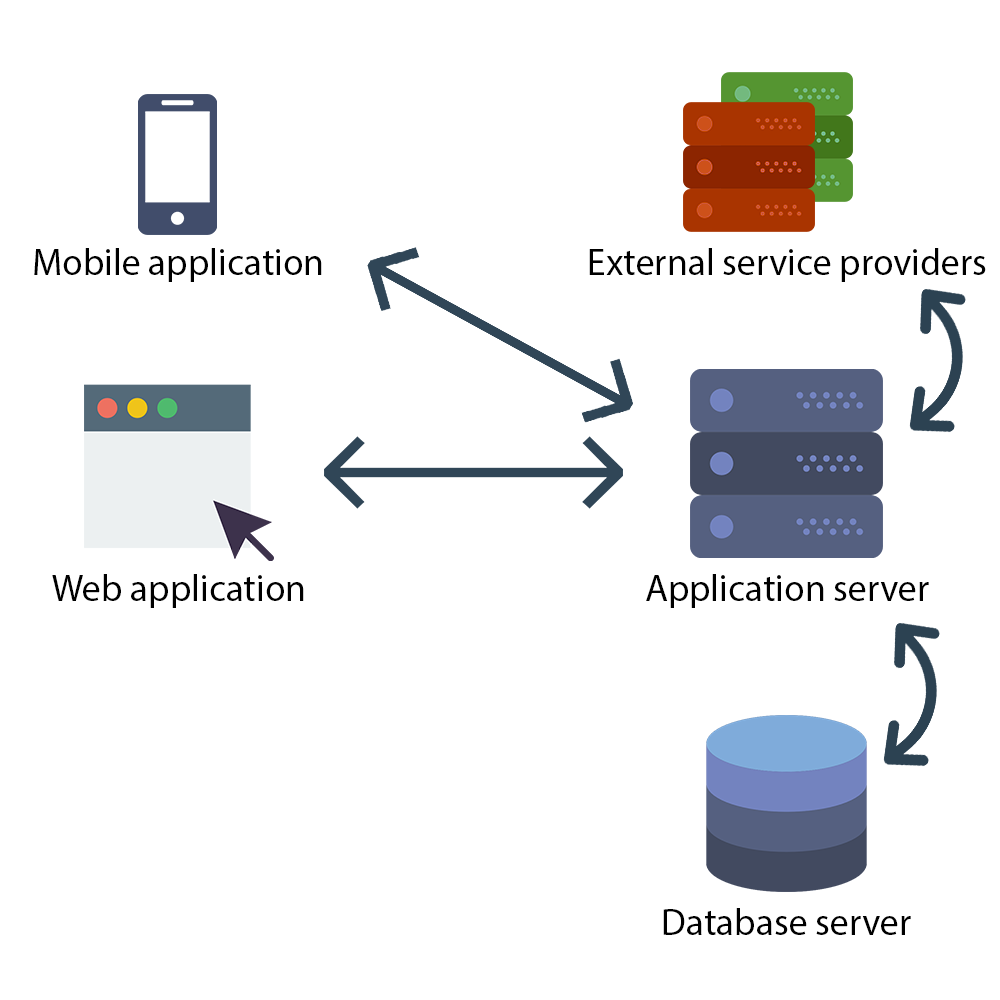
\includegraphics[width=\linewidth]{Images/Architecture/Architecture_design_2.png}
			\label{fig:Architecture}
			\end{figure}
			\paragraph{}In the development process described in the previous document, the so-called Design Document, it was taken into account that Travlendar+ will be both a mobile and web browser application. Time for developing was limited, it was established by the team to work only on the Web application. Therefore, Mobile application is considered a future expansion of the project. From the picture above it is possible to have a simplified idea of the high-level architecture, all the elements and their interactions. Regarding External Service providers, it was taken advantage of the free APIs available on the market, but it was not possible to find all the ones needed this way. So it was decided to simulate RPC calls for the services left uncovered. In the project repository there are some packages, labeled as “fake”, written down with this purpose. \\
			\paragraph{}The Application Server was entirely developed, but slightly differs from the picture: it is divided into two parts that will run in two different machines (though they will be presented into the same folder). This was done in order to be compliant with our choice of a 4-tier architecture ( see the Design Document for further details); that would lighten future mobile version developers’ job , too. With this bonds, Java EE was considered the best fit, and used for both parts. The Database Server is a normal SQL Server, while queries are handled by a JDBC Connector, provided by Spring ©. For now it was used only one database, since the amount of storage data is still low. In the future there might be one or more backups, and for management purposes a Data Warehouse. It was made sure that only beans in the back end of the Application Server could interact with the SQL one, but no security for access was provided yet.
		\subsection{Definitions, Acronyms, Abbreviations}
			\subsubsection{Definitions}
			\subsubsection{Acronyms}
			\subsubsection{Abbreviations}
			RASD : Requirement Analysis and Specification Document\\DD : Design Document\\RPC : \href{https://en.wikipedia.org/wiki/Remote_procedure_call}{Remote Procedure Call}\\API : \href{https://en.wikipedia.org/wiki/Application_programming_interface}{Application Programming Interface}\\Java EE : Java Enterprise Edition, Java Platform, Enterprise Edition (Java EE) is the standard in community-driven enterprise software.\\JB : \href{https://en.wikipedia.org/wiki/JavaBeans}{JavaBeans}\\SQL : \href{https://en.wikipedia.org/wiki/SQL}{Structured Query Language}\\JDBC : \href{https://en.wikipedia.org/wiki/Java_Database_Connectivity}{Java DataBase Connectivity}\\CDI : \href{http://www.vogella.com/tutorials/SpringDependencyInjection/article.html}{Context Dependency Injection}\\POJO : \href{https://en.wikipedia.org/wiki/Plain_old_Java_object}{Plain Old Java Object}\\IDE : \href{https://en.wikipedia.org/wiki/Integrated_development_environment}{Integrated Development Environment}\\RIA : \href{https://en.wikipedia.org/wiki/Rich_Internet_application}{Rich Internet Application}\\IoC : \href{https://en.wikipedia.org/wiki/Inversion_of_control}{Inversion of Control}
		\subsection{Revision History}
		\paragraph{} Version 1.0
		\subsection{Reference Documents}
\href{https://projects.apache.org/}{Apache Project's Documentation}\\
\href{http://vaadin.com/docs}{Vaadin Documentation}\\
Java EE - "Your First Cup: An Introduction to the Java EE Platform", Oracle 2012. \\
\href{http://spring.io/guides}{Spring}
		\subsection{Document Structure}
		\paragraph{}
The first part will be about all frameworks used in working at this project, with some screenshots and documentation. \\
The second section is about how code is divided into the different packages. It will show all the components, views, JBs, UI and so on. Some screenshots are embedded. Here it is written also about the software components designed in the DD.\\
Then in section 3 will talk about all the goals and requirements, taken from RASD, and their eventual implementation/satisfaction, evaluated according to the design “promises” of the DD . Section 4 will cover all the Testing part, while the other sections will complete the project schema with some details. To get more confident with all the frameworks and tools, it is possible to read an appendix at the end  with some background knowledge.

\newpage
	\section{Overall Description}
		\paragraph{}The project was implemented as a SpringVaadin Web Application. The programming language established for this purpose is Java 8, but some small features are written in JavaScript and HTML5.  The main reason why we chose to combine Spring with Vaadin is because it is possible to take advantage of both frameworks without any interference between the two. The main benefits were:
\begin{itemize}
\item{}It was possible to avoid working too much on HTML and CSS, but focus more on the application logic. All the code in java is translated in HTML, CSS and JavaScript by Vaadin.
\item{}Vaadin is designed to take care of all of the RIA complexity. From communication to browser quirks and rendering – it is all handled by the framework.
\item{}Easy binding to Spring data sources. It was easy to inject existing services into any part of the Vaadin UI component tree and bind the components to the data.
\item{}Thanks to Spring Boot it was possible to get a fully configured environment, including a standalone server, and to start adding content to the UI class right away.
\item{} The IoC container at the ore of Spring libraries makes it easier to write software which is more modular, reusable, maintainable and testable.
\item{}Cloudy-ready applications. Code portability through decouplng and the rich toolbox of features in Spring make it easy to forklift applications from the local development environment into any web container and cloud platform (for the future development of Travlendar+).
\item{}Spring made CDI (\textit{@Autowired}) easy to implement.
\item{}Spring has a wide range of useful libraries.
\end{itemize}
\paragraph{}To get a deeper understanding of these modern concepts of web design, such as IoC, CDI and so on, we suggest to look at the links proposed in the Reference Documents section and skim the Appendix. However, a simplified snapshot of the code will be given here.\\
In Vaadin server-side applications, all pages to be shown to the clients are loaded dynamically in one singleton instance of the class UI (custom UIs like in this project extends it). Anytime a client connects to the server a dedicated UI is instantiated. This UI containts a "navigator" object that allows navigation of the various contents. The navigator is called anytime certain events are triggered: a click for example, or when some response must be shown. The various pages are java classes that are initialized by the navigator. All web components, such as text fields, cheboxes and images, are defined in pages, that act like views in a Model-View-Presenter pattern. In the code of these classes, which can be found in the package \textit{com.polimi.travlendar.frontend.pages} (see the following section), it is possible to embed Java Beans, Spring Components and Services, that elaborate all the data input given by clients and are responsible of the application business logic. This connection is made possible by the tag \textit{@Autowired}, provided by Spring, similarly to some JavaEE tags. This brief description can be completed by reading the sections on Vaadin and Spring in the appendix.
\newpage
	\section{Structure of the source code}
		\begin{figure}[H]
		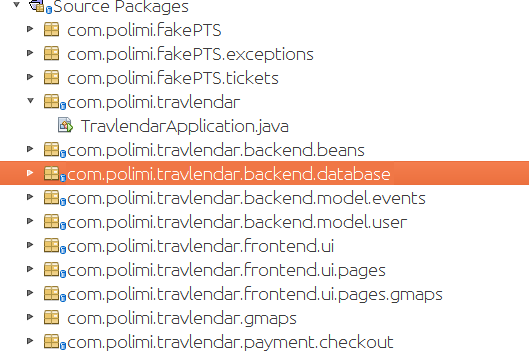
\includegraphics[width=\linewidth]{Images/source_code_structure.png}
		\label{fig:Source Code}
		\end{figure}
			\paragraph{}
The picture above displays the packages and their organization. FakePTS folder represents the simulation of a generic Public Transportation System's java API (such as \textit{ATM}, \textit{AMT}, etc...). It contains all the classes and methods to generate valid tickets (which are POJOs) and validate them electronically.\\ The Spring Boot Application starter class is called \textit{TravlendarApplication} and is in the main folder \textit{travlendar}. Running it from any Java IDE will start the application. The code of the application is divided into two subfolders: \textit{backend} and \textit{frontend}.\\The first one hosts the code that will be deployed in the Application Server, which includes the model of the objects necessary for the functionalities, along with the Business tier (the Beans). It also contains the folder \textit{database}, where all the elements to extract and insert data into the DB server are contained.\\The latter contains all the elements for the user interface: the UI class, the classes for the web pages and other UI components.\\The package \textit{gmap} contains all the elements to enhance the dialogue with the Google Maps API and services, while the \textit{checkout} package contains the code for the collaboration with Stripe APIs.\\In the picture below it is possible to se the modules that were defined in the DD:
 		\begin{figure}[H]
		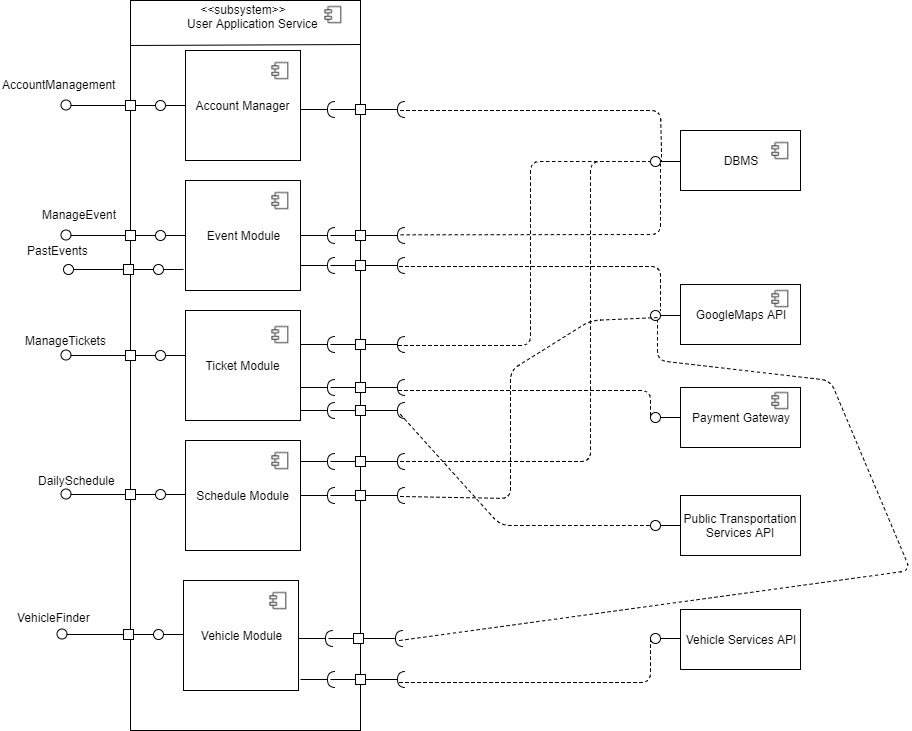
\includegraphics[width=\linewidth]{Images/Architecture/User_Application_Service.png}
		\label{fig:Modules}
		\end{figure}
			\paragraph{}
Each module of the subsystem \textit{User Application Service} was implemented in the same way: one single session bean with all the methods to handle requests formulated by the front end components, backed up by some model elements. Therefore, modules are not visible in the packages' structure at first sight. For example, the first module on top \textit{Account Manager} is made of the bean named \textit{UserService} and some calsses in the model folder such as \textit{User}, \textit{UserSettings}, \textit{UserPreferences} etc..\\The external modules (shown on the right side of the picture) were defined independently and can easily be mapped 1:1 with the packages described above.\\The module \textit{Vehicle Module} was not implemented into the project.
\newpage
		\subsection{Pages}
			\subsubsection{Login/Register}
		\paragraph{}This section will show screenshots of the website's pages.
			\begin{figure}[H]
			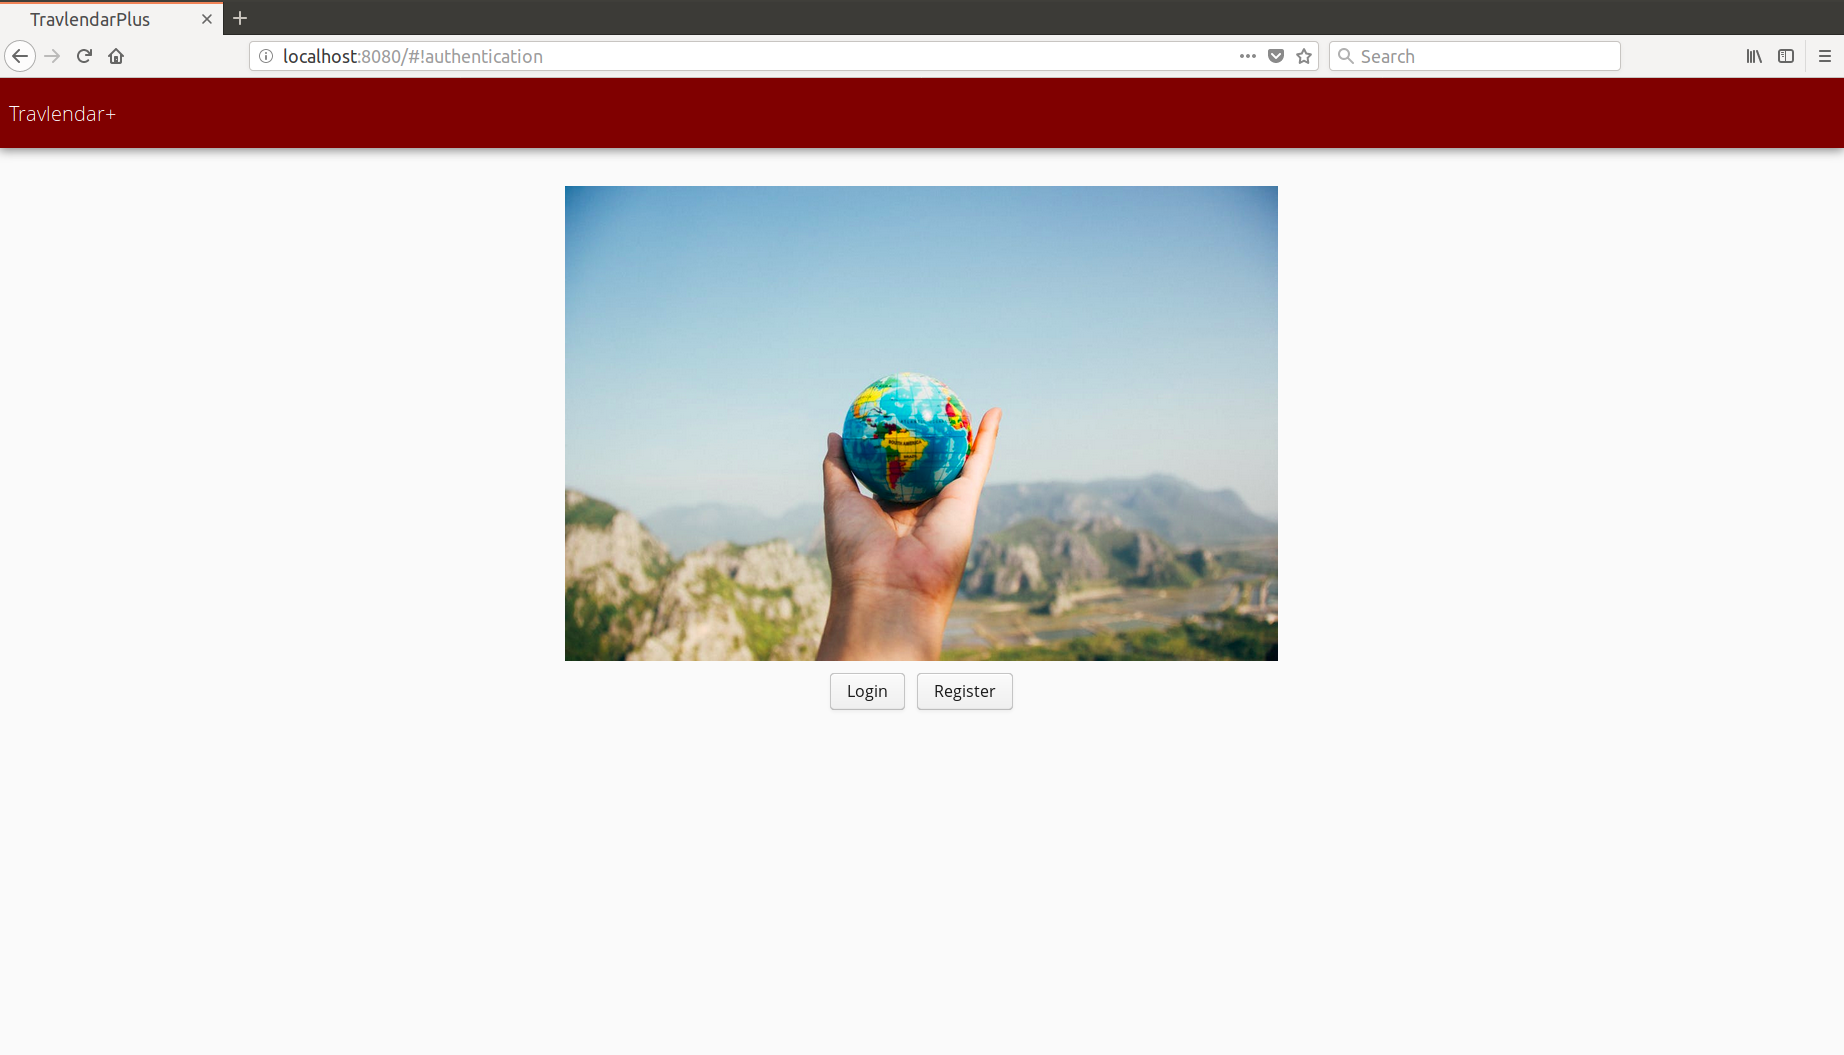
\includegraphics[width=\linewidth]{Images/Pages/1-Login.png}
			\label{fig:Login}
			\end{figure}
		This is the first page that will appear when the application is started. It allows registration and login.
			\subsubsection{Map}
			\begin{figure}[H]
			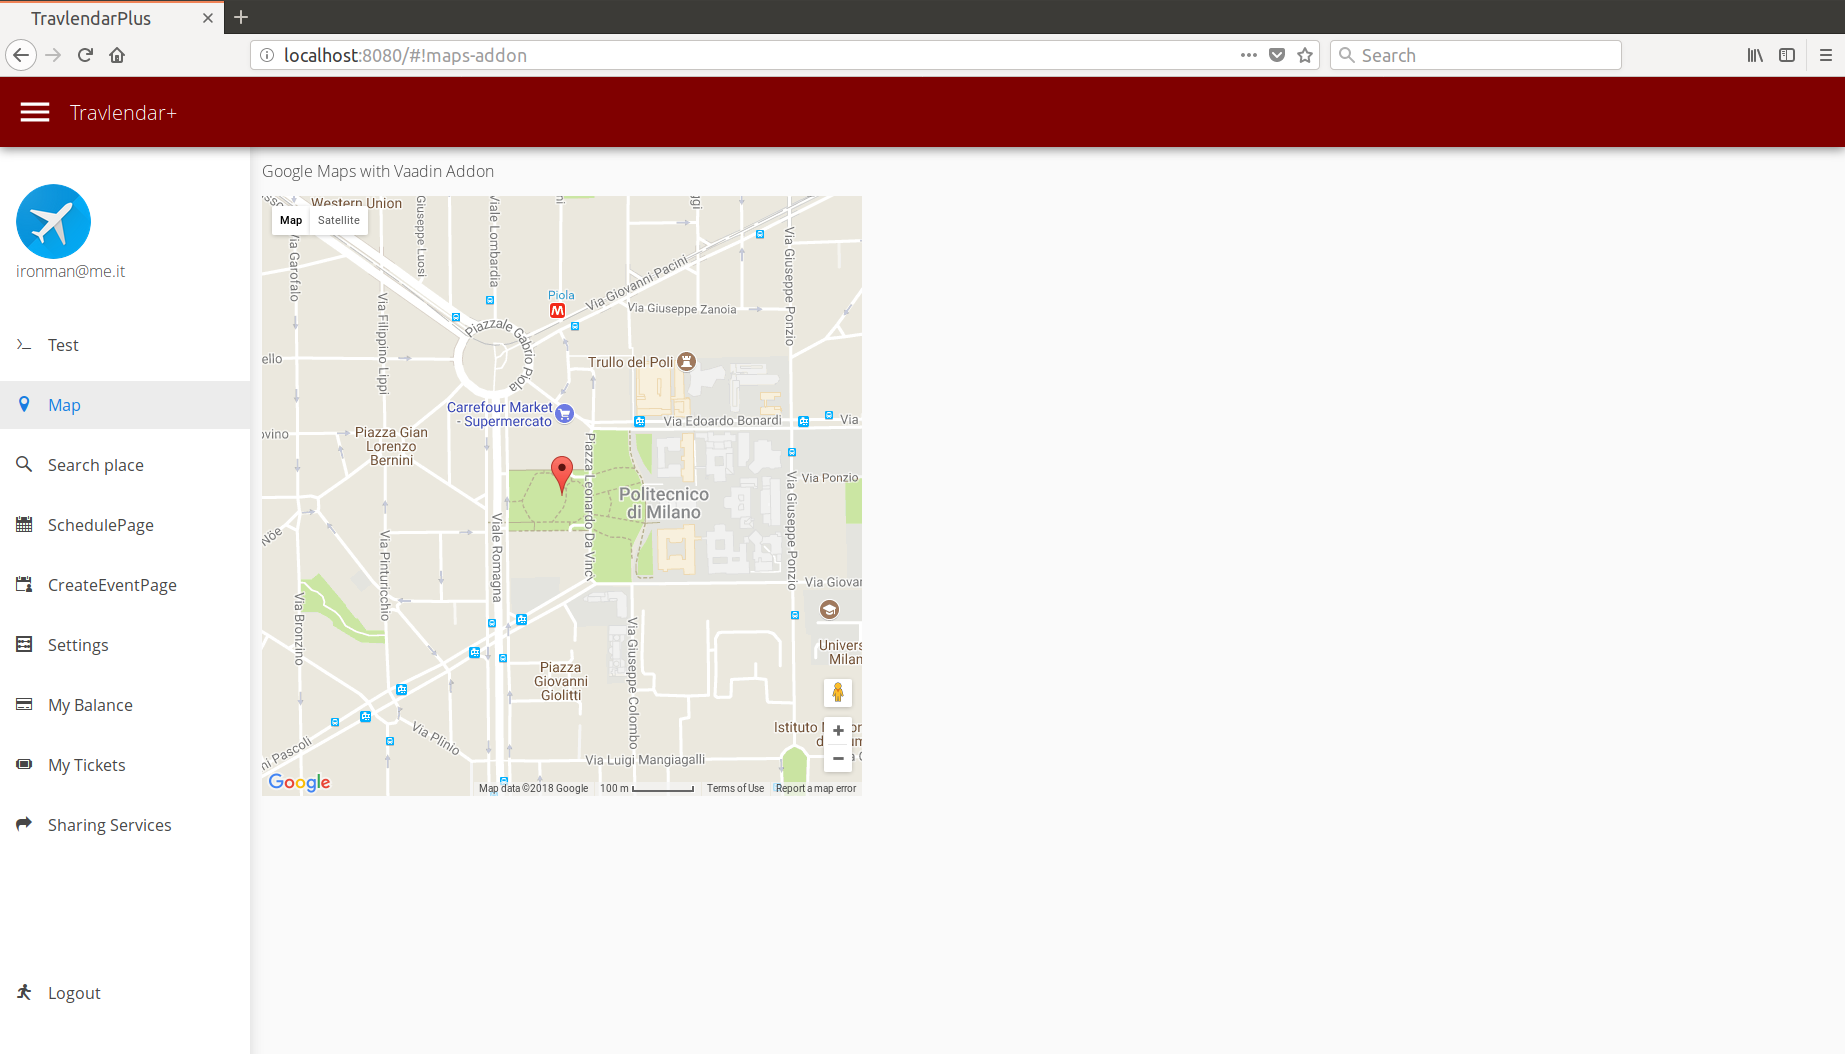
\includegraphics[width=\linewidth]{Images/Pages/2-Map.png}
			\label{fig:Map}
			\end{figure}
		Once logged in, the menu bar appears on the left, showing all the pages of the website. The first one is the map: here the user can see his roundabouts.
			\subsubsection{Place Search}
			\begin{figure}[H]
			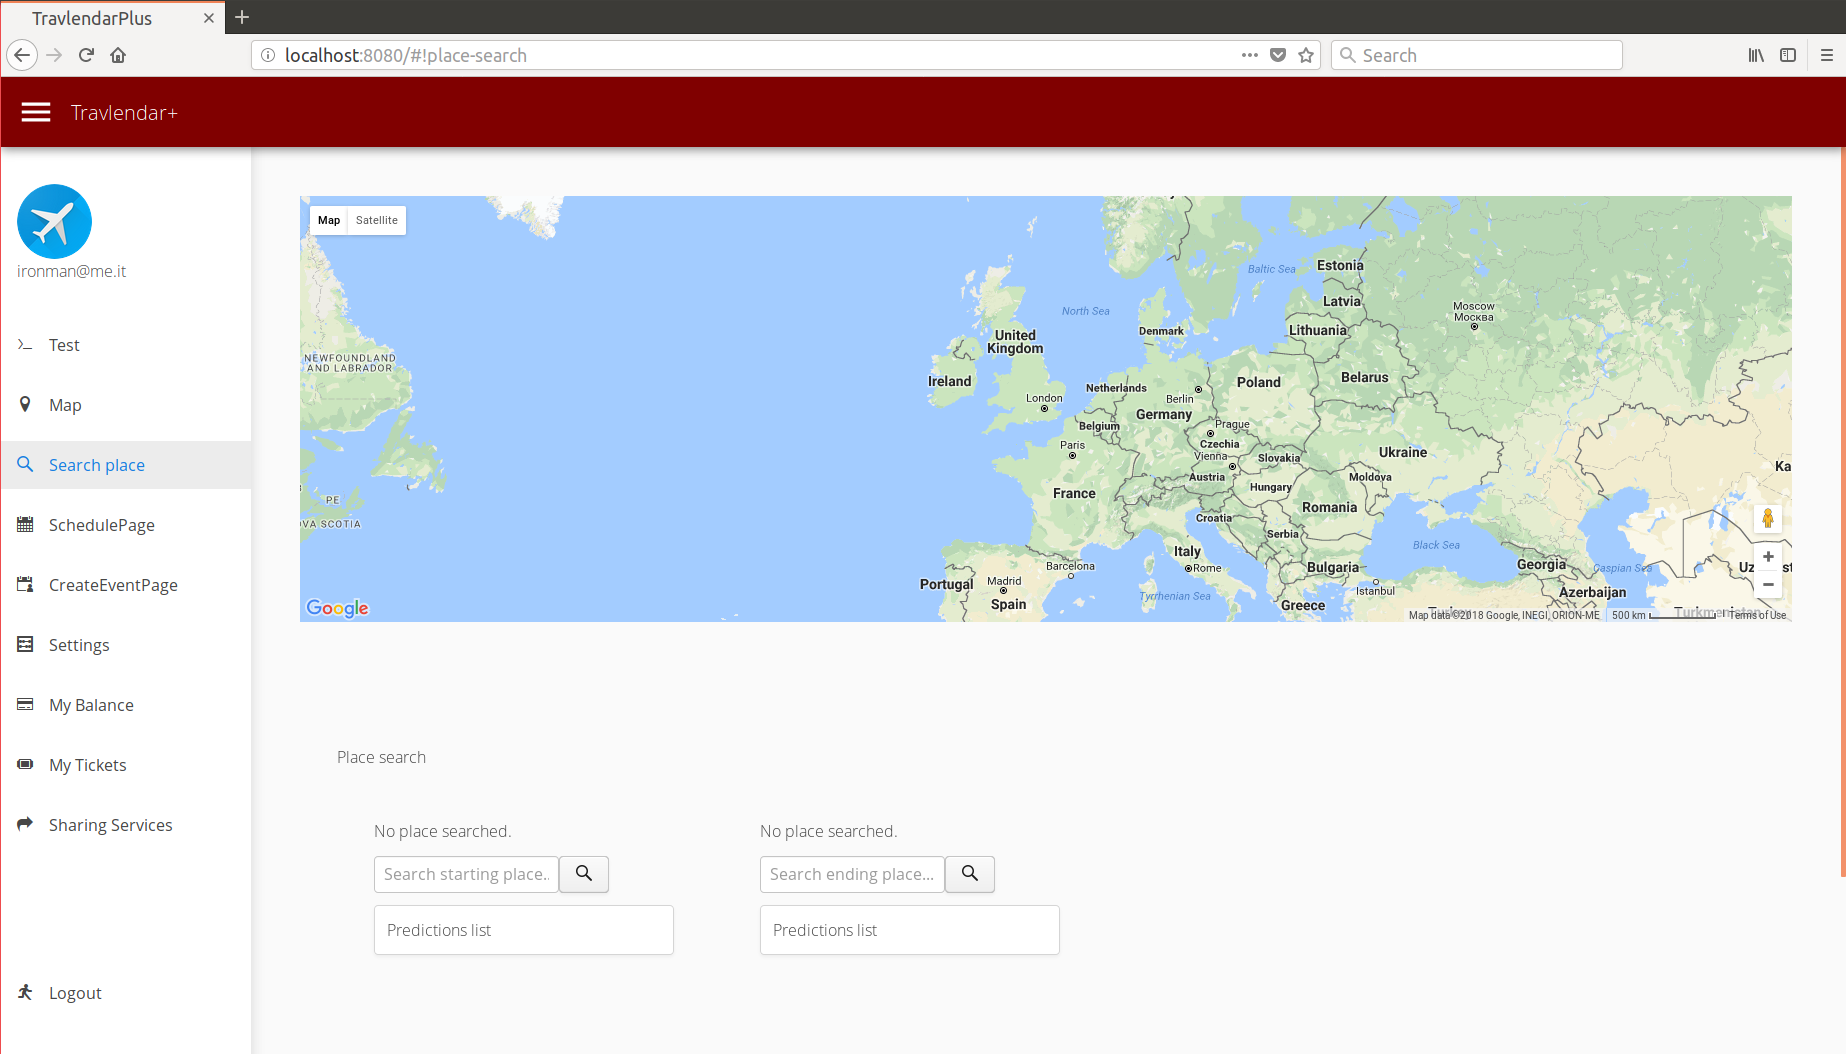
\includegraphics[width=\linewidth]{Images/Pages/3-Map.png}
			\label{fig:Map2}
			\end{figure}
		The second page is for place search.
			\subsubsection{Schedule}
			\begin{figure}[H]
			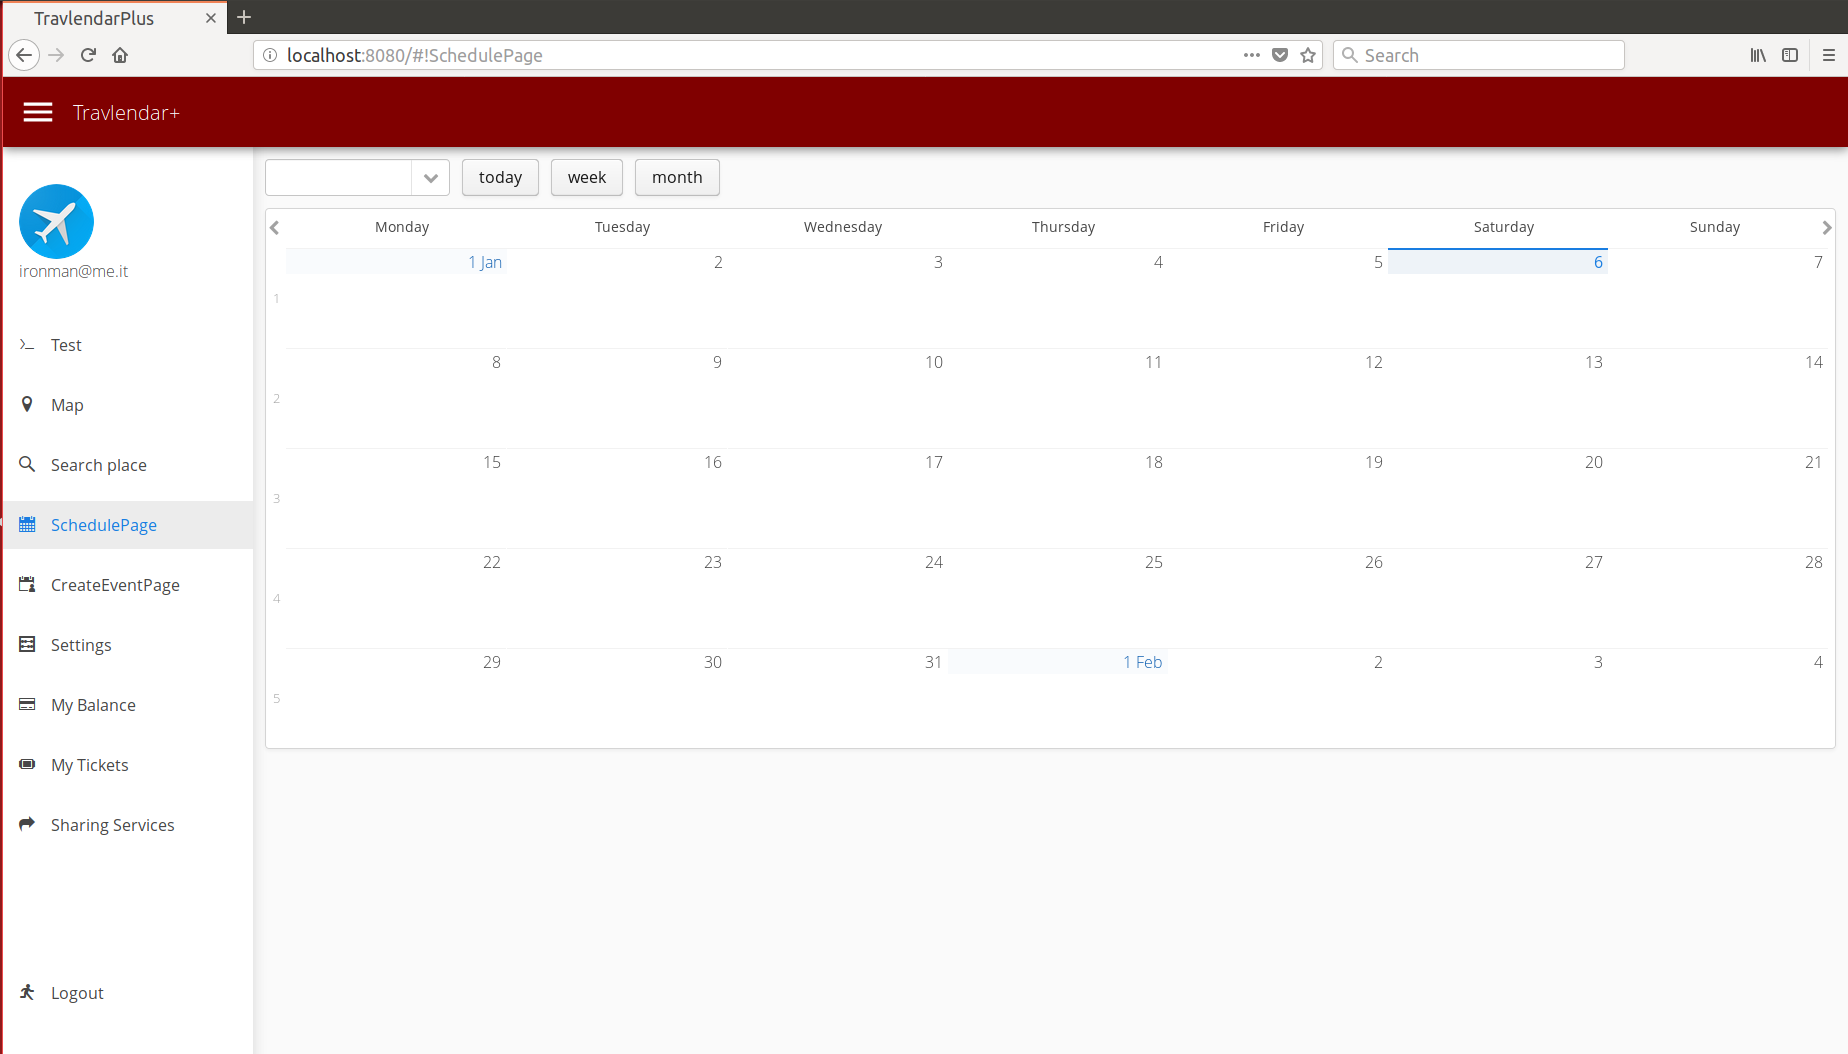
\includegraphics[width=\linewidth]{Images/Pages/4-Schedule.png}
			\label{fig:Schedule}
			\end{figure}
		The third page contains the schedule. Here the user can see his agenda and the events he created. Selecting an event with the mouse will give you the option to modify or delete it.
			\subsubsection{Create Event}
			\begin{figure}[H]
			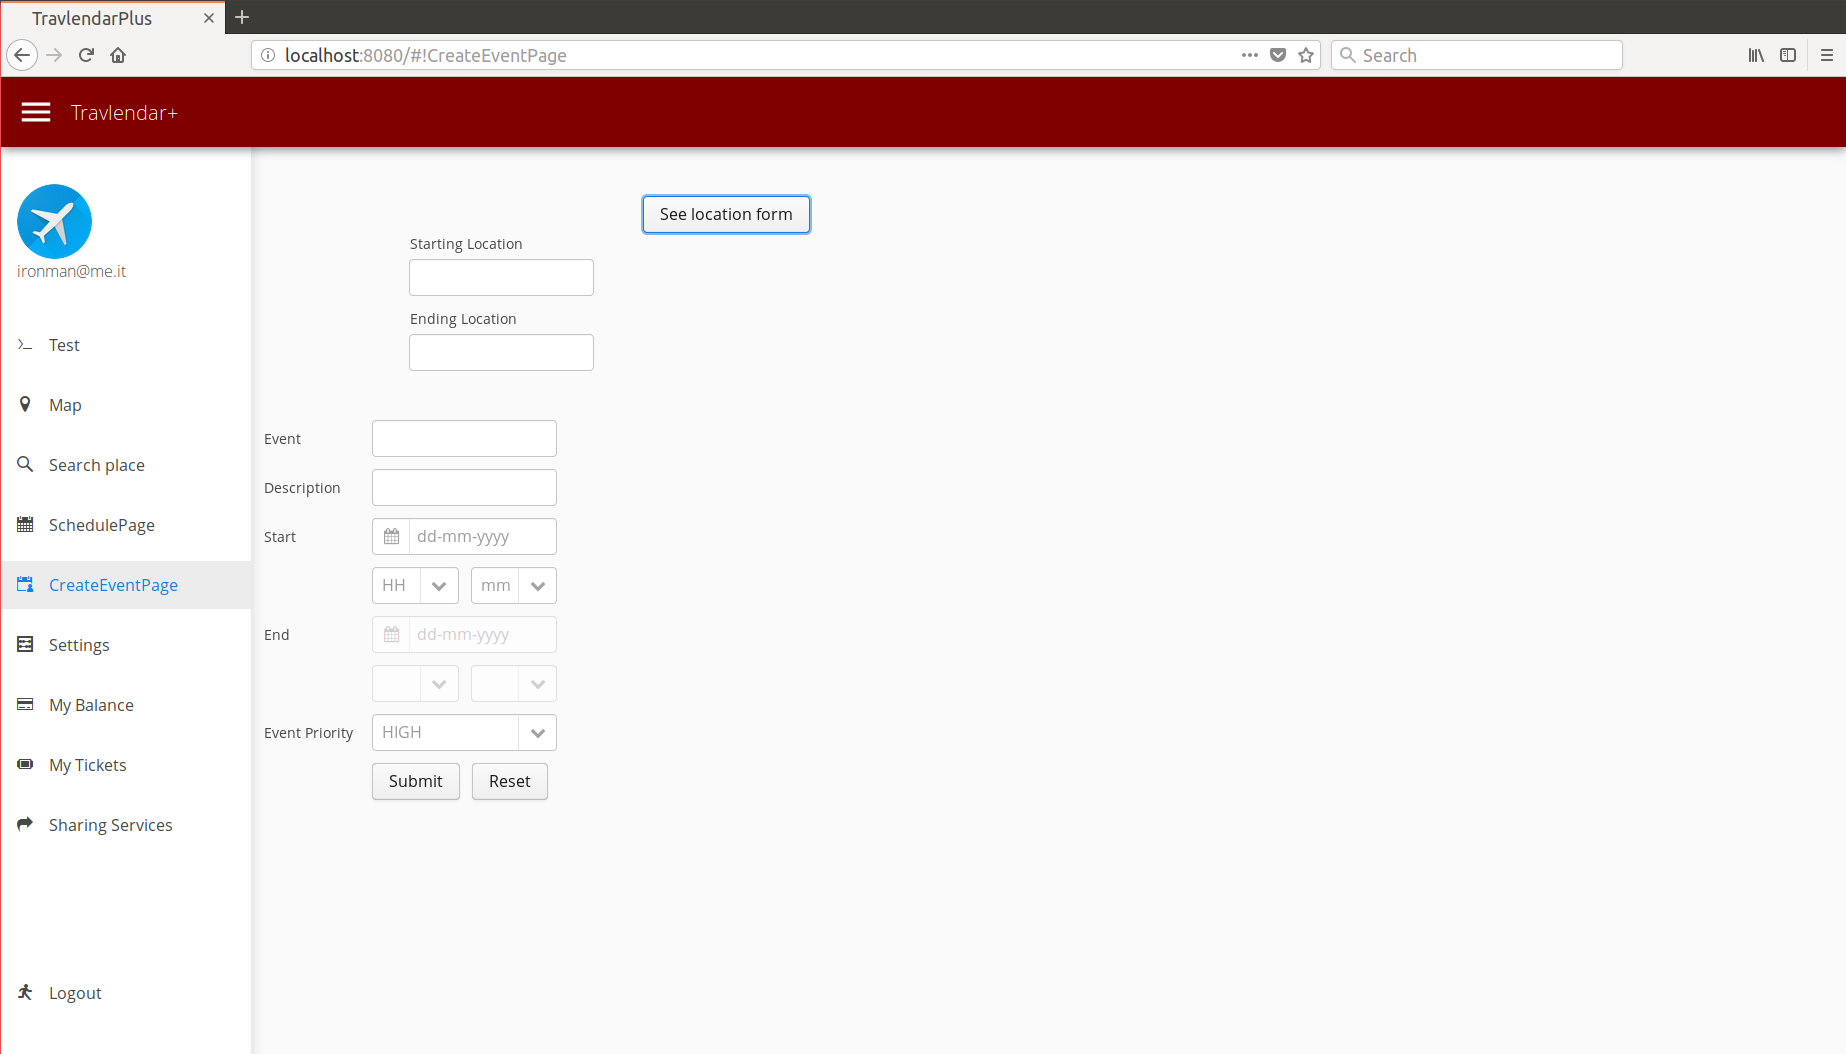
\includegraphics[width=\linewidth]{Images/Pages/5-Create_Event.png}
			\label{fig:Create_Event}
			\end{figure}
		In this page the user can create new events. By clicking on the \textit{See location form} a window pops up with the possibility of selecting where you will be located when you head out to go to the event and where the event will be.
			\subsubsection{Preferences}
			\begin{figure}[H]
			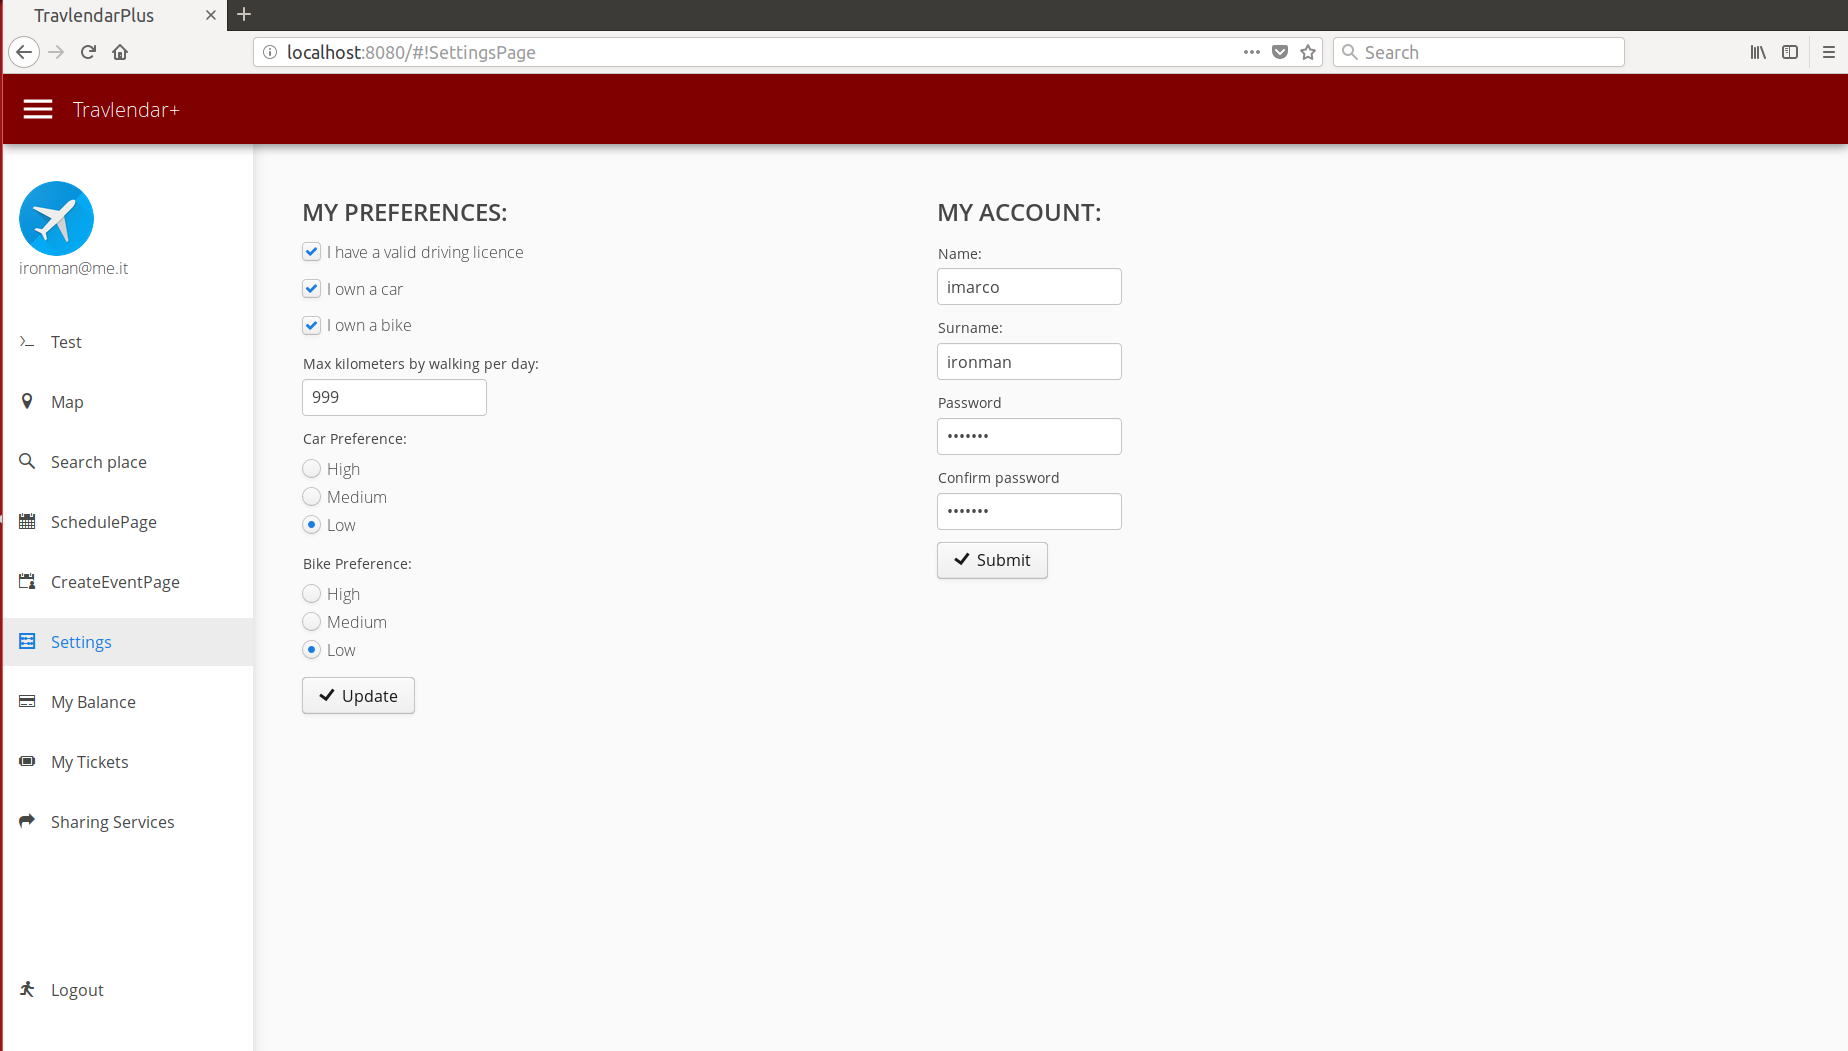
\includegraphics[width=\linewidth]{Images/Pages/6-Preferences.png}
			\label{fig:Preferences}
			\end{figure}
		Here are loaded all the user's customizable preferences and account details. Update and Submit buttons will make the system save the selected ones.
			\subsubsection{Balance}
			\begin{figure}[H]
			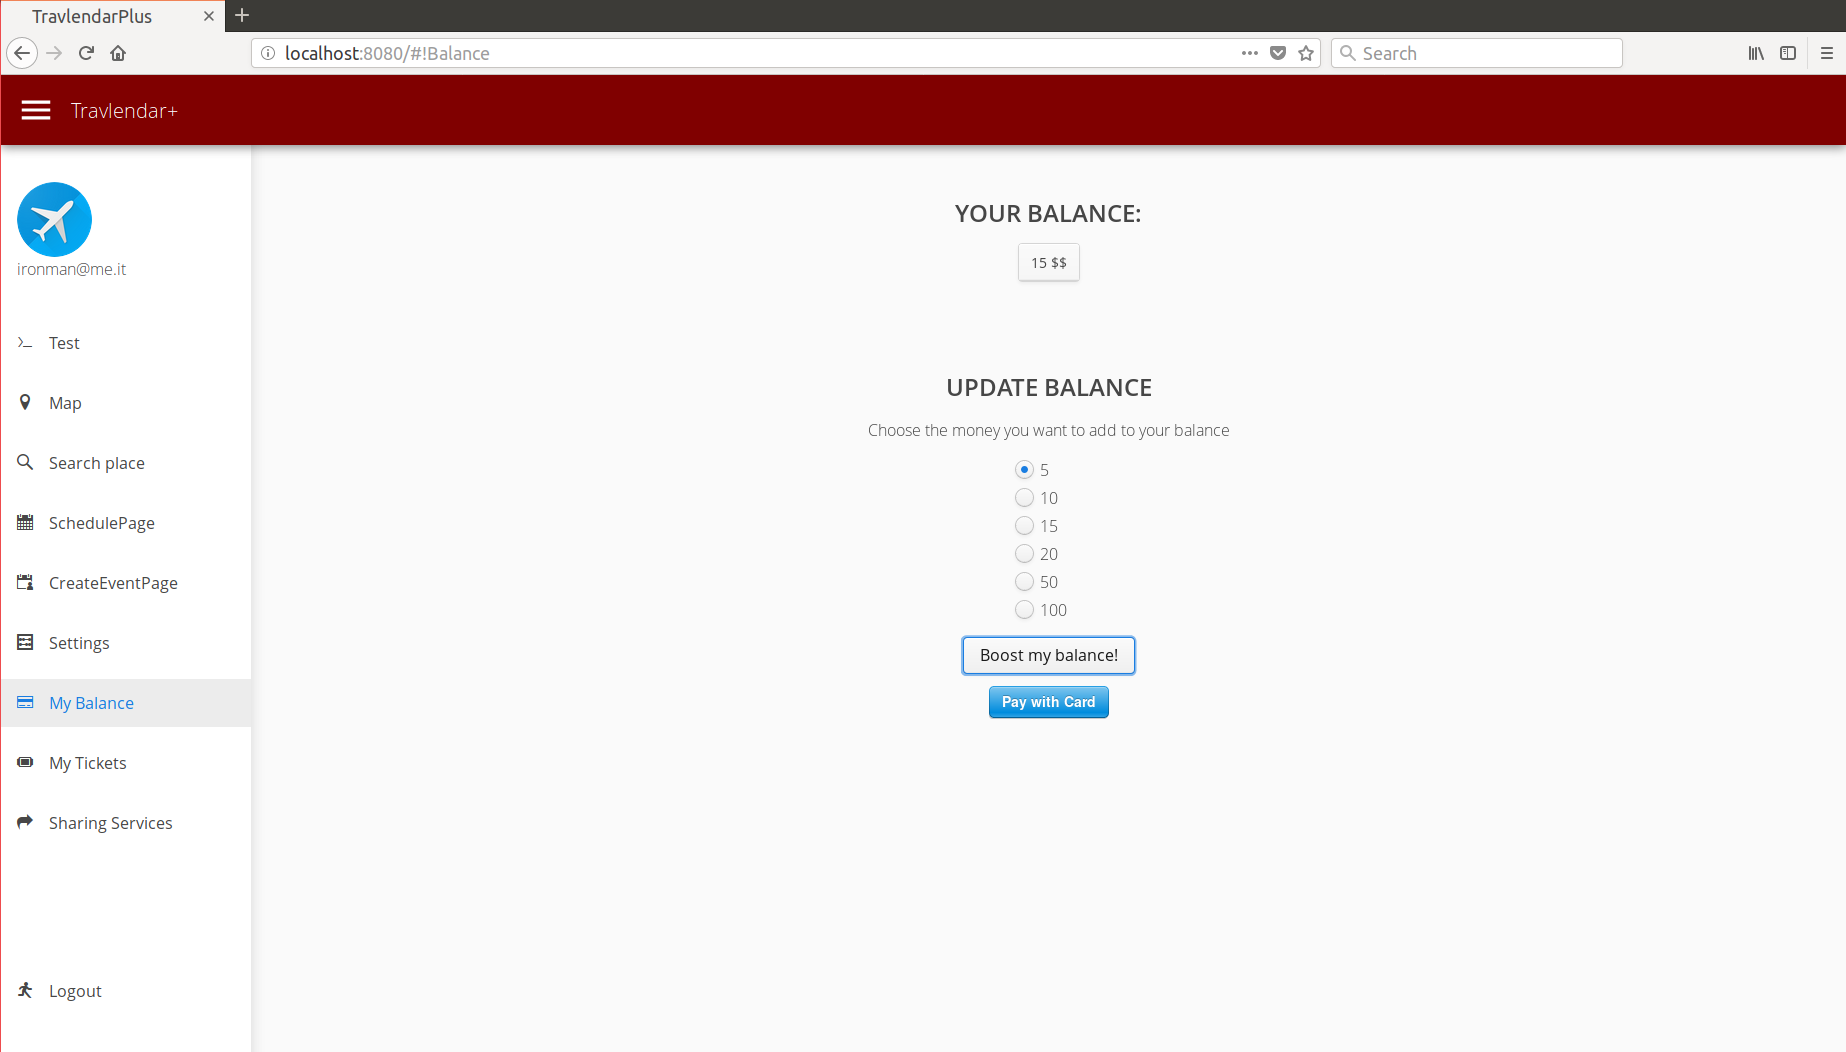
\includegraphics[width=\linewidth]{Images/Pages/7-Balance.png}
			\label{fig:Balance}
			\end{figure}
	My Blanace Page concerns Travlendar's currency. Every user will have a balance which can be increased by clicking on \textit{Pay with Card} and filling all the credit card required fields that pop up afterwards.
			\subsubsection{Tickets}
			\begin{figure}[H]
			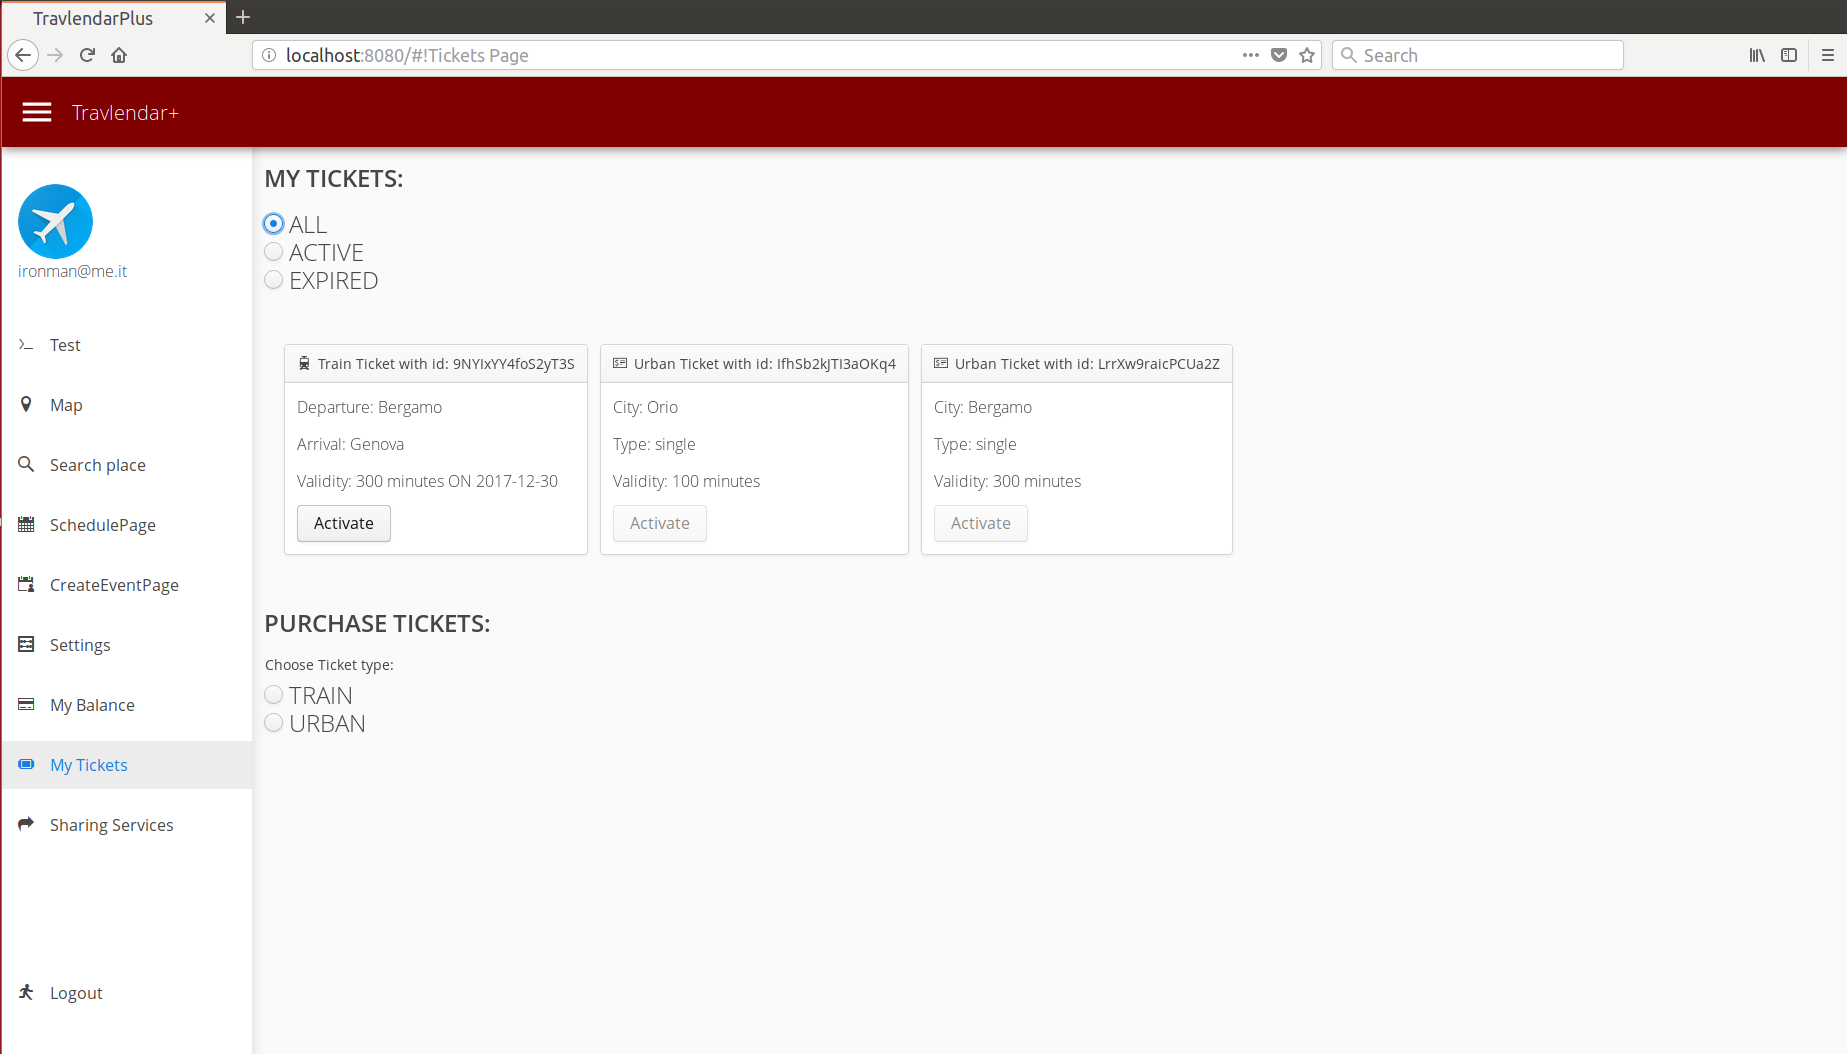
\includegraphics[width=\linewidth]{Images/Pages/8-Tickets.png}
			\label{fig:Tickets}
			\end{figure}
		This is the area where it is possible to purchase tickets through the application (balance currency is needed for this operation) and to access the ones owned (that may be active or not).
			\subsubsection{Sharing Services}
			\begin{figure}[H]
			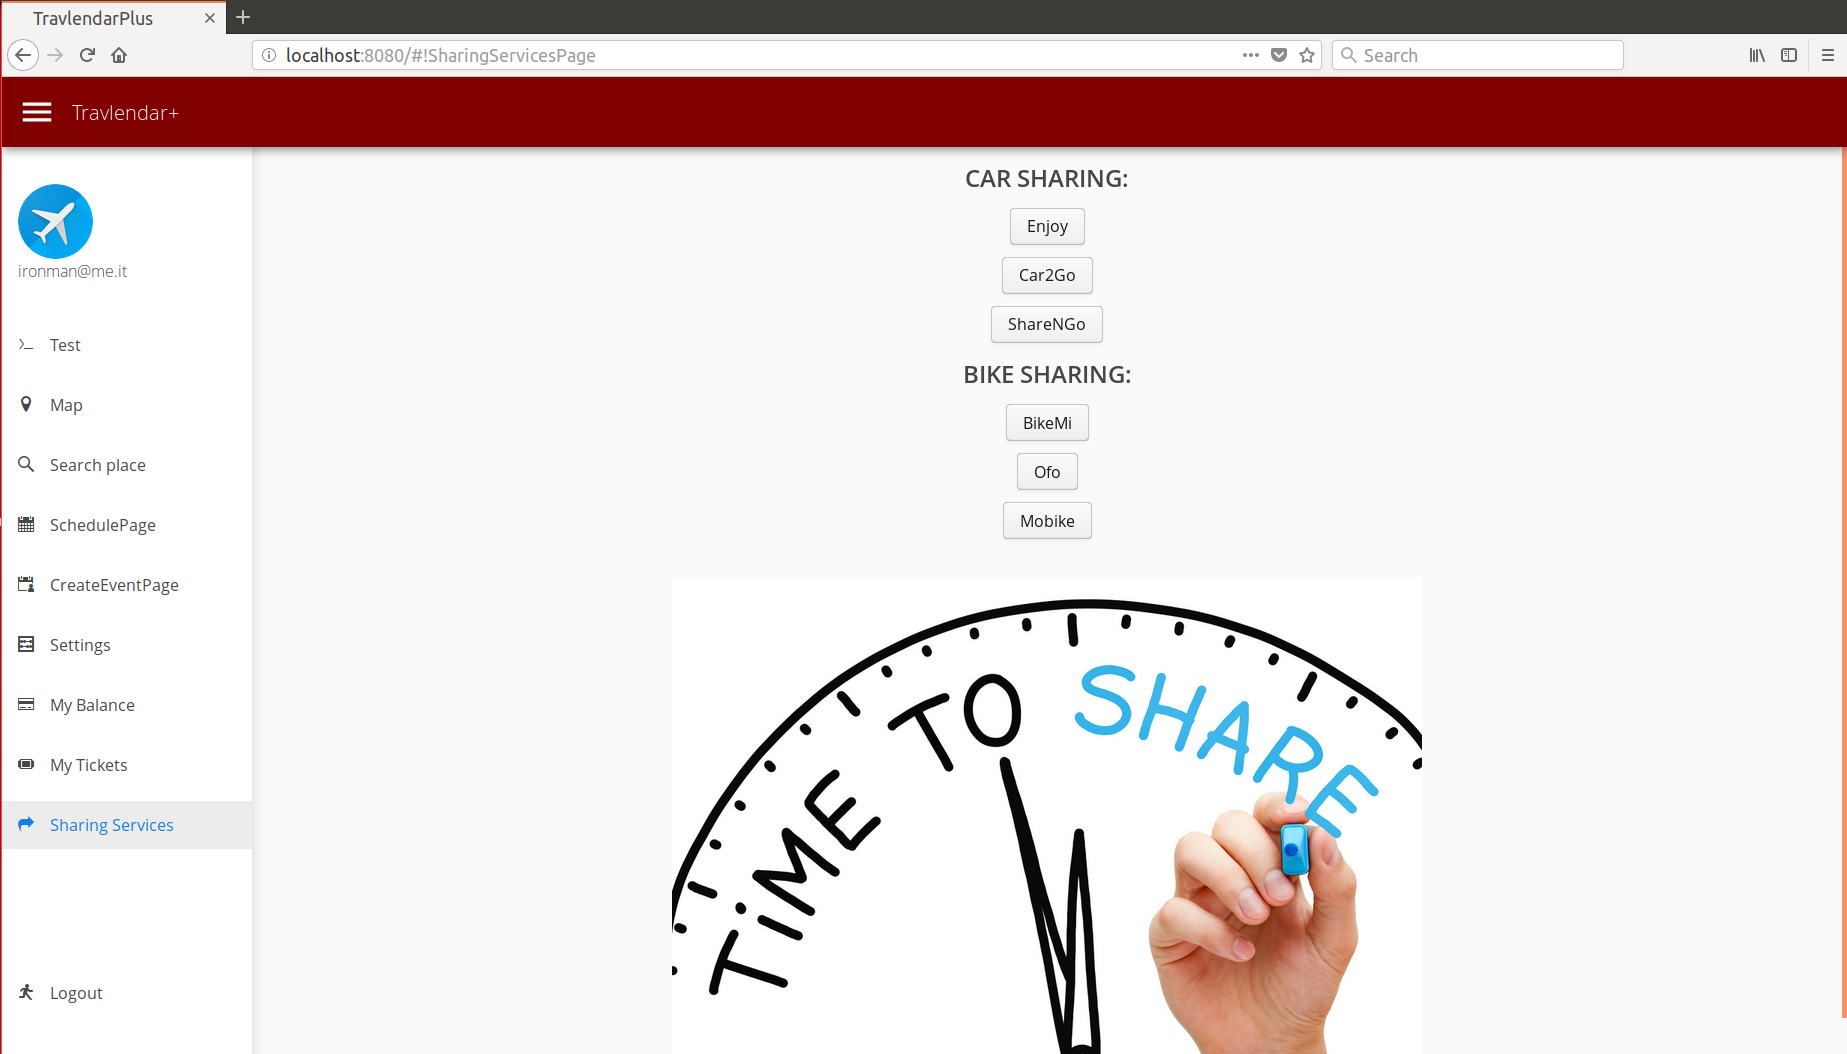
\includegraphics[width=\linewidth]{Images/Pages/9-CSS.png}
			\label{fig:Sharing Services}
			\end{figure}
		The last page is to advertise the car and bike sharing services Travlendar+ has agreements with. In the future this page will directly show vehicles on the map.
\newpage
	\section{Requirements and Functionalities}
		\subsection{Functional Requirements}
		\paragraph{}In this section we will map the first prototype of Travlendar+ with all the goals and requirements, specified in the RASD, in order to highlights which functionalities are ready-to-use and which ones will be implemented or improved in the future.
			\subsubsection{Goal 1}
			\begin{figure}[H]
			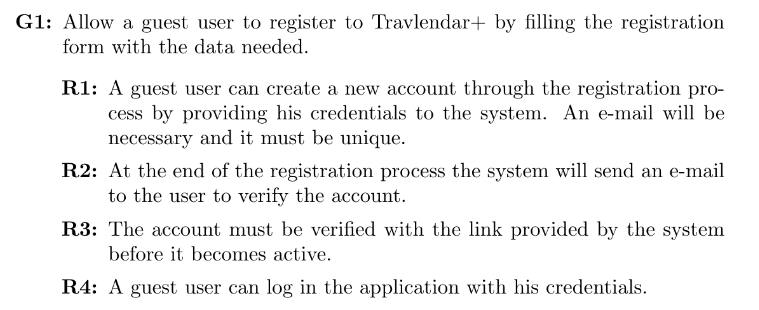
\includegraphics[width=\linewidth]{Images/Goals/Goal_1.png}
			\label{fig:G1}
			\end{figure}
		\paragraph{}The application has its own register/login component that works. For now only input data are verified and not personal email existence. We didn't configure a server mail yet, which means that the system does not send a confirmation email but immediately registers the new user into the database.
			\subsubsection{Goal 2}
			\begin{figure}[H]
			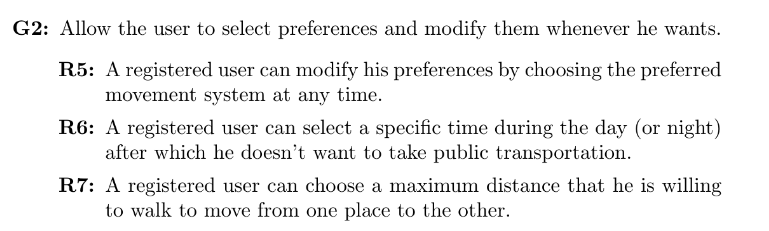
\includegraphics[width=\linewidth]{Images/Goals/Goal_2.png}
			\label{fig:G2}
			\end{figure}
		\paragraph{}Travlendar+ contains a dedicated page, called \textit{Settings Page}, where the user can customize his preferences. All the requirements are satisfied.
			\subsubsection{Goal 3}
			\begin{figure}[H]
			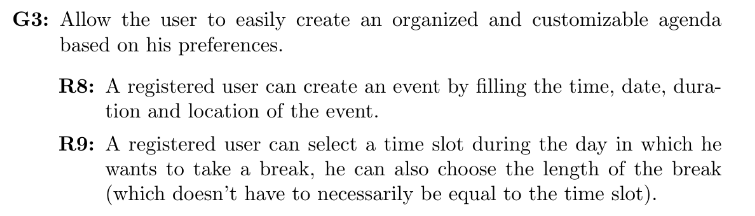
\includegraphics[width=\linewidth]{Images/Goals/Goal_3.png}
			\label{fig:G3}
			\end{figure}
		\paragraph{}This goal has been achieved, the application contains a calendar in which users can create events and modify them, by giving the application the information about where they will be before going to the event, where the event will be, and the starting and ending time of the event. Lunch breaks are considered a future development feature.
			\subsubsection{Goal 4}
			\begin{figure}[H]
			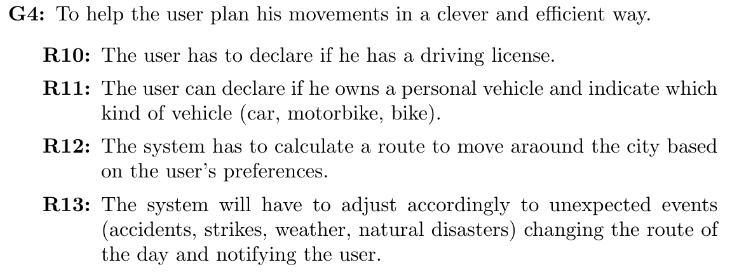
\includegraphics[width=\linewidth]{Images/Goals/Goal_4.png}
			\label{fig:G4}
			\end{figure}
		\paragraph{}The algorithm for path suggestion is not optimal, but it still gives the fastest path to the selected location. The other requirements are achieved.
			\subsubsection{Goal 5}
			\begin{figure}[H]
			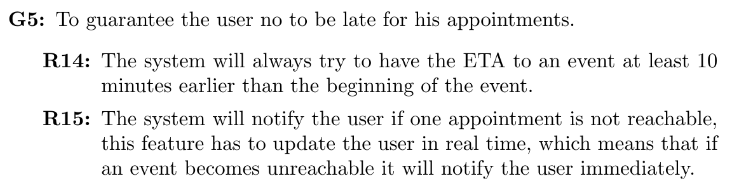
\includegraphics[width=\linewidth]{Images/Goals/Goal_5.png}
			\label{fig:G5}
			\end{figure}
		\paragraph{}This goal was not achieved and will be developed in the future. The system does currently deal with real time changes.
			\subsubsection{Goal 6}
			\begin{figure}[H]
			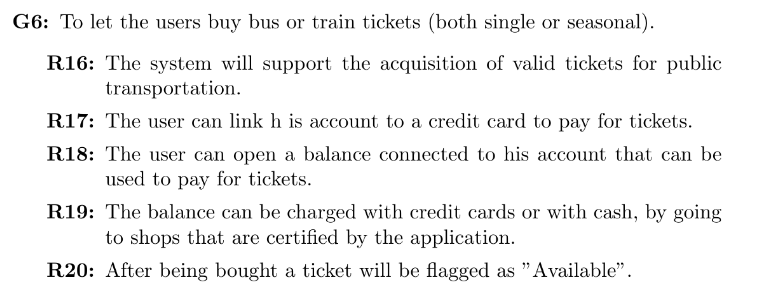
\includegraphics[width=\linewidth]{Images/Goals/Goal_6.png}
			\label{fig:G6}
			\end{figure}
		\paragraph{}This goal has been achieved. The application has a page in which the user can buy new tickets that can be used. Even though the PTS APIs are faked, the system is open and ready for a real collaboration about payments. The credit and debit cards are not saved in the database, the user will have to submit the details everytime. Tickets can be purchased only with Travlendar+'s balance value. This way all the money transactions pass through the system (in particulare the payment gateway module).
			\subsubsection{Goal 7}
			\begin{figure}[H]
			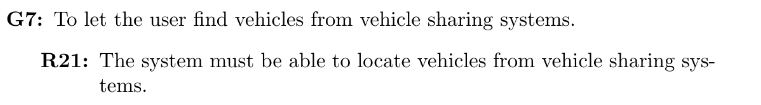
\includegraphics[width=\linewidth]{Images/Goals/Goal_7.png}
			\label{fig:G7}
			\end{figure}
		\paragraph{}This feature was not implemented. At the moment the application will redirect the user to external websites of different car and bike sharing systems.
			\subsubsection{Goal 8}
			\begin{figure}[H]
			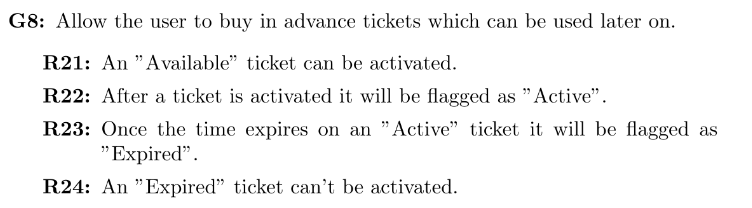
\includegraphics[width=\linewidth]{Images/Goals/Goal_8.png}
			\label{fig:G8}
			\end{figure}
		\paragraph{}This goal has been achieved. Tickets are stored in Travlendar+'s databases and can be activated at any moment after their purchase. The expiration is handled too.
		\subsection{Non-functional Requirements}
			\begin{figure}[H]
			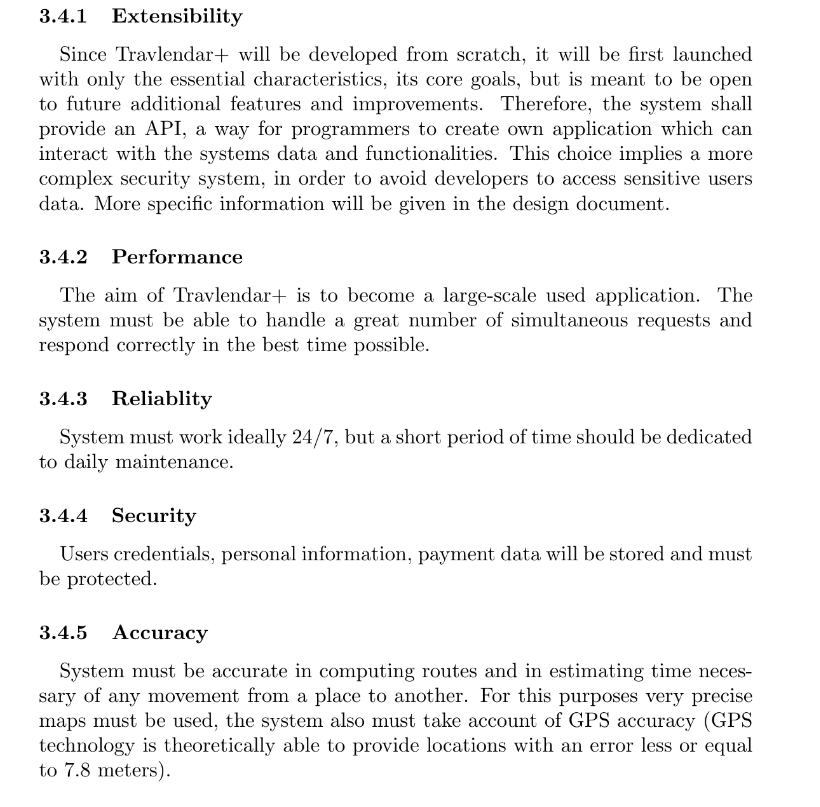
\includegraphics[width=\linewidth]{Images/Goals/Non-functional_requirements.png}
			\label{fig:G8}
			\end{figure}
		\paragraph{}Regarding non-functional requirements, the project has successfully satisfied the first three. The code is shareable on open-source, can ideally run non-stop and does not generate performance issues. The other two have not been implemented only because we didn't have to deal with them yet. They are flagged as open issues, but the developers are confident that with a little improvement they can be easily achieved.
\newpage
	\section{Testing}
\newpage
	\section{Installation Instruments}
		\subsection{Configuration}
		\paragraph{In short\\}Import in your IDE as a Maven project. \\You need to execute mvn install. Some IDEs (e.g.: Eclipe JEE) automatically execute it when you run the project.
Run the class TravlendarApplication.java as a Java Application.\\From your browser navigate to localhost:8080.
		\subsection{Database Configuration with MySQL Workbench}
		\paragraph{}To import the database in your PC:
		\begin{enumerate}
			\item Install MySQL Workbench.
			\item In the program: Server -$>$ Data Import.
			\item Select "Import from Self-Contained File" and browse Dump.sql.
			\item Create a new schema for the Default Target Schema and name it "travlendar" (important).
			\item Refresh schemas to see travlendar.
		\end{enumerate}
		\subsection{Database Configuration with Command Line}
		\paragraph{}Alternately, create manually a new schema with MySQL Command Line:\\Copy and Paste commands from the file \textit{"sql\_entries"} that is accessible in the folder \textit{Implementation}.
		\subsection{Configure JDBC}
		\paragraph{}To access the database, the application reads the information in the file \textit{src/main/resources/application.properties}. By default, the application tries to connect to localhost:3306 with username "admin" and password "root", which are the standard settings of MySQL Workbench.


\newpage
	\section{References}
\begin{itemize}
\item{}\href{https://vaadin.com/blog/building-a-web-ui-for-mysql-databases-in-plain-java-?utm_campaign=New%20registration&utm_source=hs_automation&utm_medium=email&utm_content=39610603&_hsenc=p2ANqtz--ut22Rfm32KlobpIHtq6LpH3COcrPL4sZEWDAXO1ZoRH34i0P46KUYGkVxwFIw49_cBYJPSgFVZ82j3sQ5lAAvDc8h-g&_hsmi=39610603}{Vaadin + MySQL}
\item{}\href{https://vaadin.com/docs/v8/framework/layout/layout-overview.html}{Vaadin layout components}
\item{}\href{https://vaadin.com/docs/v8/framework/application/application-overview.html}{Vaadin server-side app}
\item{}\href{https://www.w3schools.com/sql/default.asp}{SQL Syntax}
\item{}\href{https://examples.javacodegeeks.com/enterprise-java/vaadin/vaadin-login-example/}{Vaadin login}
\item{}\href{https://www.petrikainulainen.net/programming/maven/integration-testing-with-maven/}{Integration testing in Maven}
\item{}\href{https://www.petrikainulainen.net/programming/maven/creating-code-coverage-reports-for-unit-and-integration-tests-with-the-jacoco-maven-plugin/}{Jacoco}
\item{}Testing in Spring: the following documents
\\ 	\href{https://docs.spring.io/spring/docs/current/spring-framework-reference/testing.html}{https://docs.spring.io/spring/docs/current/spring-framework-reference/testing.html}
\\ 	\href{http://www.baeldung.com/spring-boot-testing}{http://www.baeldung.com/spring-boot-testing}
\\ 	\href{https://techbeacon.com/how-extend-java-unit-tests-components-spring-mockito}{https://techbeacon.com/how-extend-java-unit-tests-components-spring-mockito}
\item{}\href{http://www.evosuite.org/documentation/maven-plugin/}{EvoSuite Maven Plugin Tutorial}
\item{}\href{http://www.baeldung.com/java-stripe-api}{Stripe for Spring}
\item{}\href{https://vaadin.com/directory/component/app-layout-add-on}{App-Layout Vaadin Addon Documentation}
\end{itemize}			
\newpage
	\section{Effort Spent}
		\begin{itemize}
			\item{Team work:} $\sim$ 120 hours.
			\item{Individual work:} $\sim$ 110 hours each.
		\end{itemize}

\appendix
\newpage
	\section{Background Knowledge}
		\paragraph{}In this section we provide an idea of the usage of all the main frameworks and software tools which are responsible of Travlendar+ first prototype's shape and code. We will also give an insight on the impact each framework had on the project.
		\subsection{Apache Maven}
		\paragraph{}Apache Maven is a software project management and comprehension tool. Based on the comncept of a project object model (POM), Maven can manage a project's build, reporting and documentation from a central piece of information. Maven's primary goal is to allow a developer to comprehend the complete state of a development effort in the shortest period of time. In order to attain this goal there are several areas of concern that Maven attempts to deal with:
\begin{itemize}
\item{}Making the build process easy.
\item{}Providing an uniform build system.
\item{}Providing quality project information.
\item{}Providing guidelines for best practices development.
\item{}Allowing transparent migration to new features.
\end{itemize}
		\paragraph{Version:} 3.5.2
		\paragraph{Advantages:}
		\begin{itemize}
			\item{}It was very easy for the developers to add APIs, Vaadin Elements, Spring features and all kind of pre-built packages.
		\end{itemize}
		\paragraph{Drawbacks:}
		\begin{itemize}
			\item{}None in our project.
		\end{itemize}
		\paragraph{In our project:}see pom.xml file in the code's folder.
	\subsection{Vaadin}
			\begin{figure}[H]
			\begin{center}
			
\includegraphics[width=0.2\linewidth]{Images/Appendix/vaadin1.png}
			\label{fig:V1}
			\end{center}
			\end{figure}

			\paragraph{}Vaadin Framework is a Java web application development framework that is designed to make creation and maintenance of high quality web-based user interfaces easy. Vaadin supports two different programming models: server-side and client-side. The server-driven programming model is the more powerful one. It lets you forget the web and program user interfaces much like you would program a desktop application with conventional Java toolkits such as AWT, Swing, or SWT. But easier.\\
			\paragraph{}While traditional web programming is a fun way to spend your time learning new web technologies, you probably want to be productive and concentrate on the application logic. The server-side Vaadin framework takes care of managing the user interface in the browser and the AJAX communications between the browser and the server. With the Vaadin approach, you do not need to learn and deal directly with browser technologies, such as HTML or JavaScript. (Read more at \href{https://vaadin.com/docs/v8/framework/introduction/intro-overview.html}{https://vaadin.com/docs/v8/framework/introduction/intro-overview.html})
			\begin{figure}[H]
			\begin{center}
			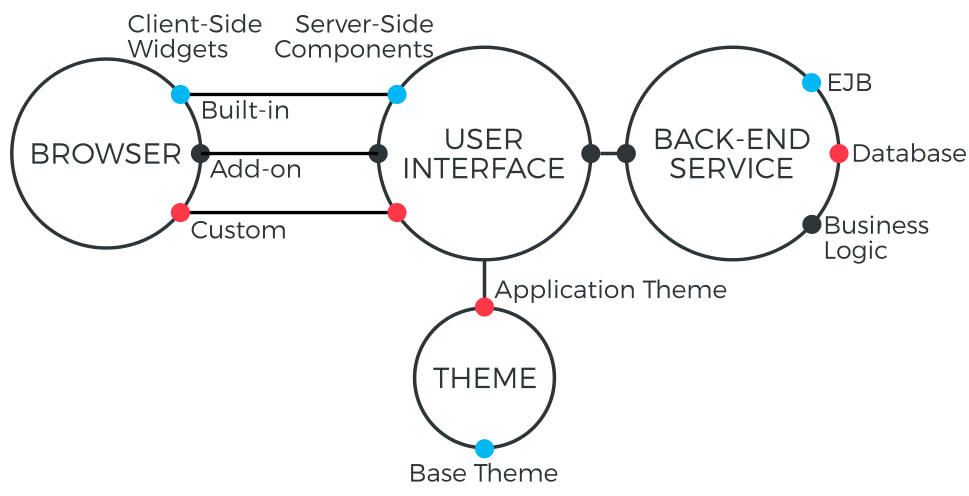
\includegraphics[width=.8\linewidth]{Images/Appendix/vaadin2.png}
			\label{fig:V2}
			\end{center}
			\end{figure}
			\paragraph{}Vaadin Framework consists of a server-side API, a client-side API, a horde of user interface components/widgets on the both sides, themes for controlling the appearance, and a data model that allows binding the server-side components directly to data. For client-side development, it includes the Vaadin Compiler, which allows compiling Java to JavaScript.
			\begin{figure}[H]
			\begin{center}
			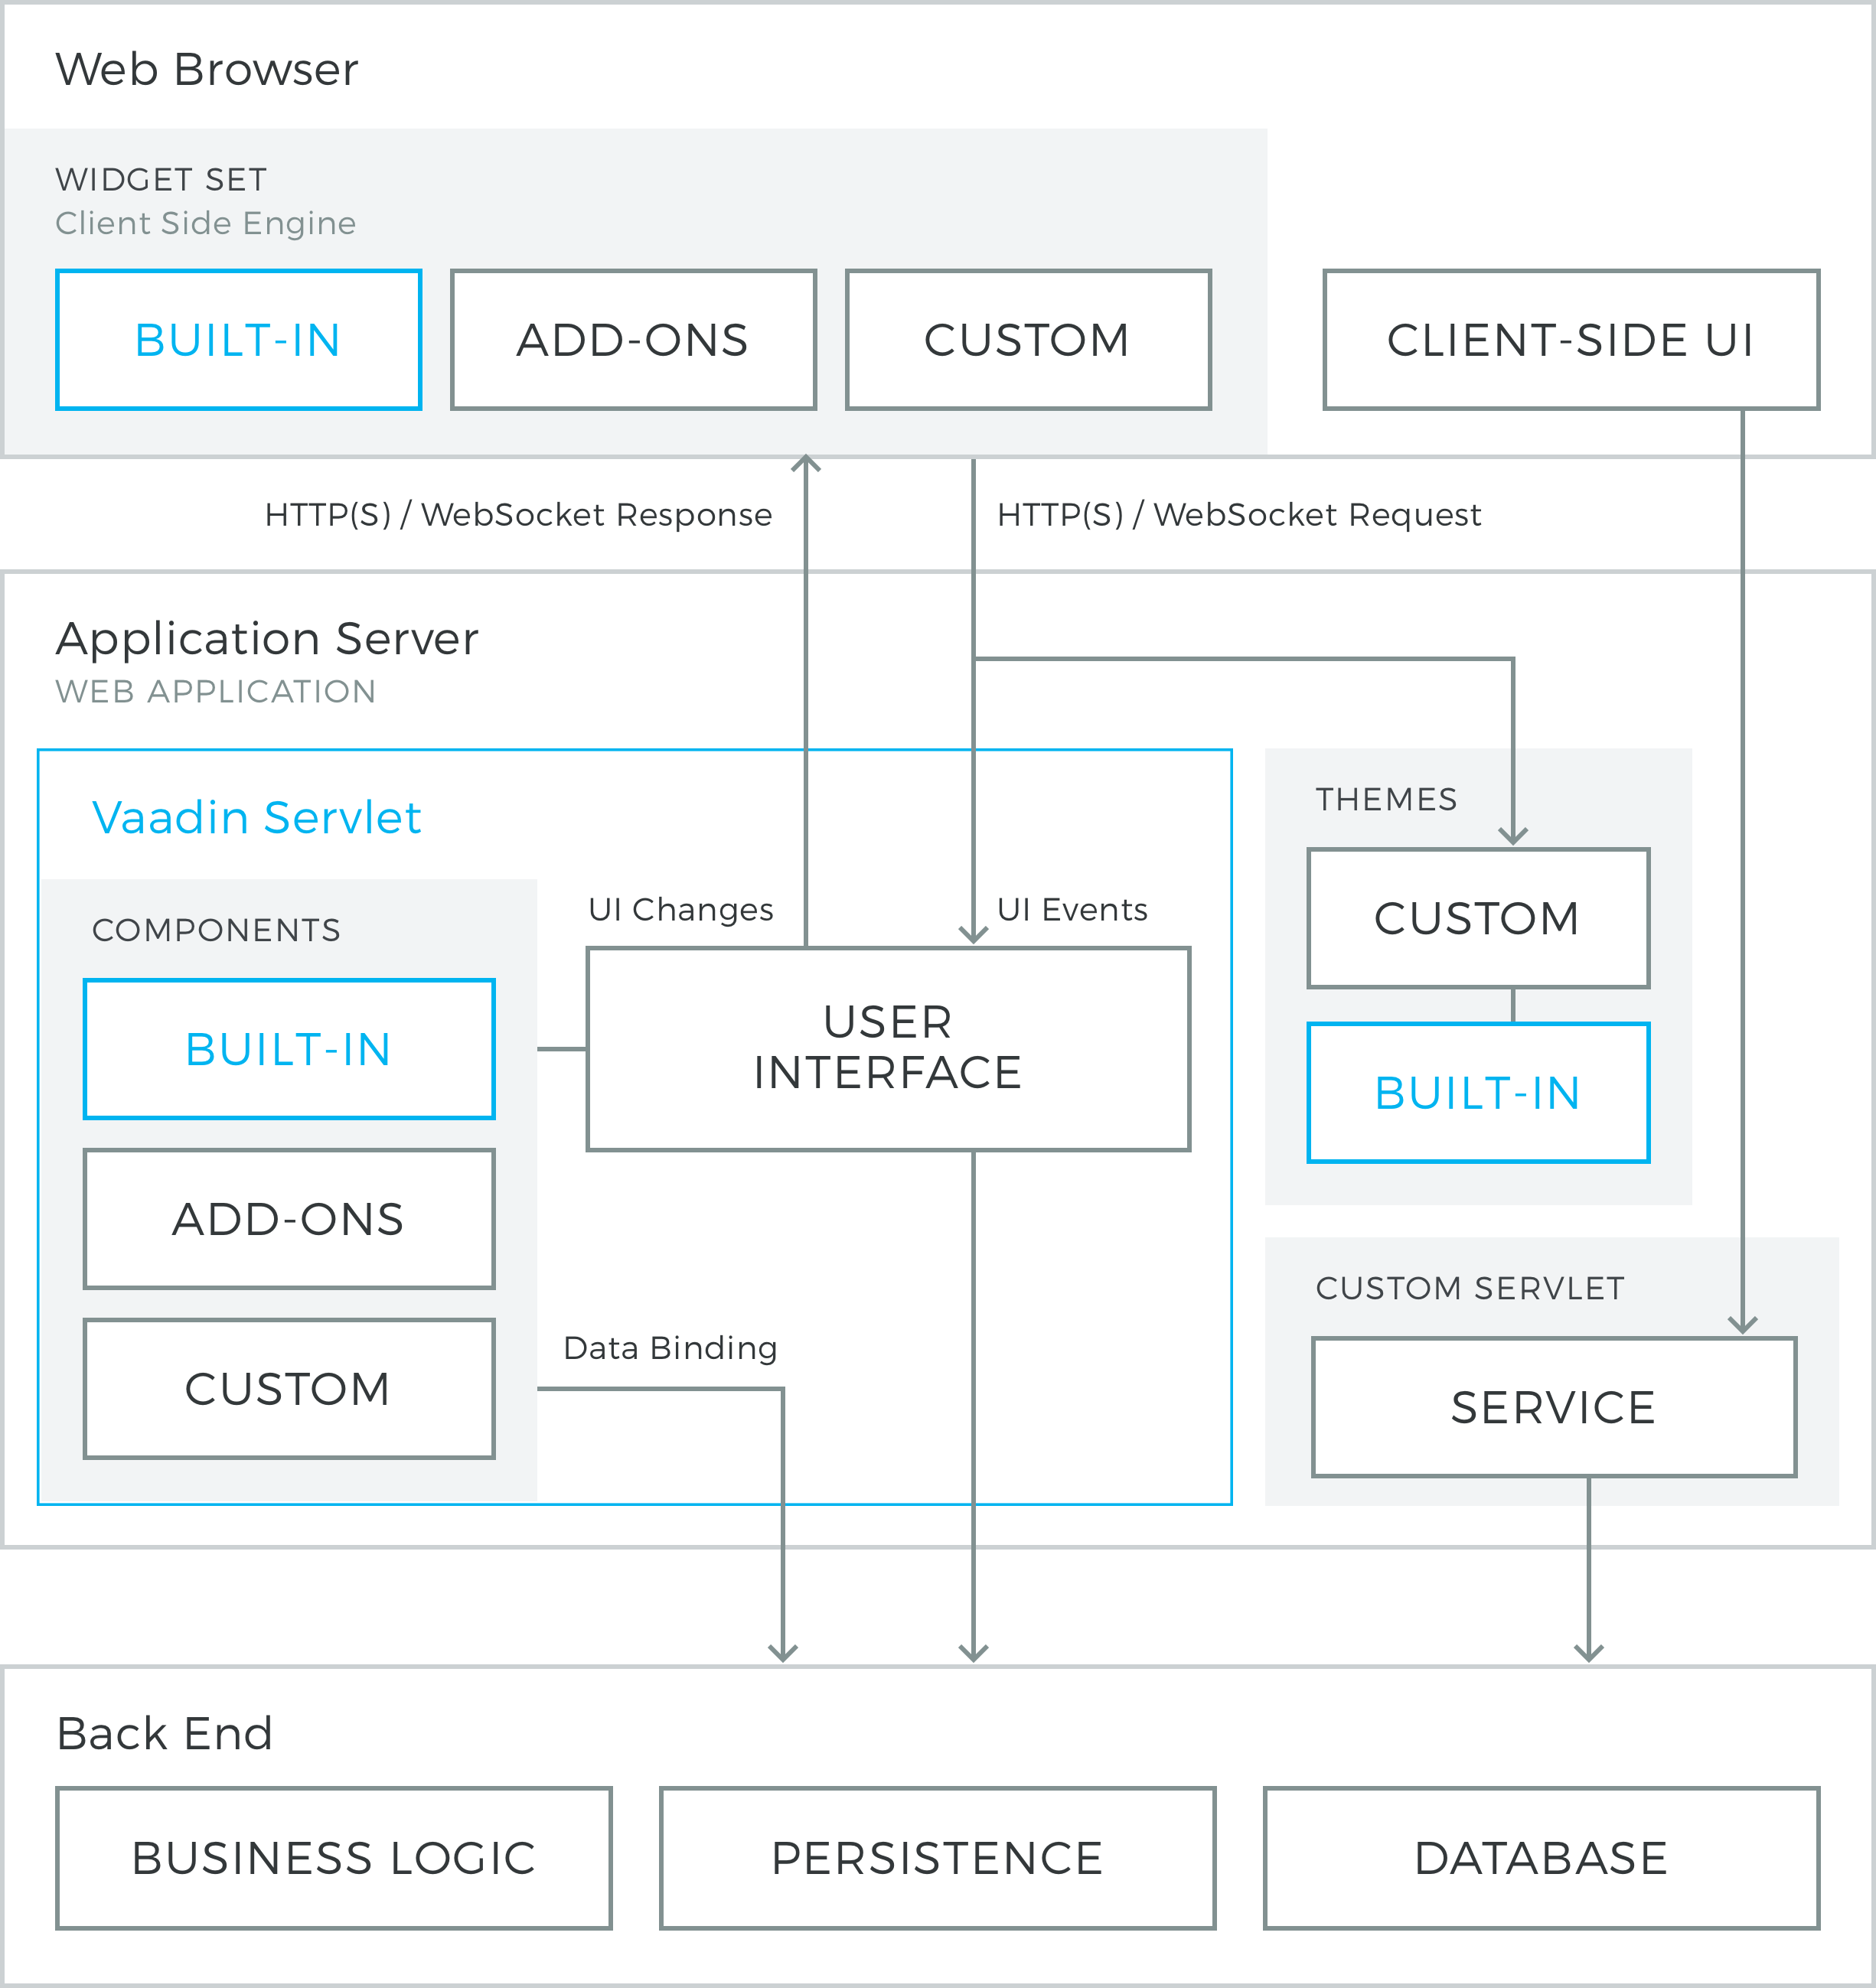
\includegraphics[width=.8\linewidth]{Images/Appendix/vaadin4.png}
			\label{fig:V4}
			\end{center}
			\end{figure}
			\paragraph{}A server-side Vaadin application runs as a servlet in a Java web server, serving HTTP requests. The VaadinServlet is normally used as the servlet class. The servlet receives client requests and interprets them as events for a particular user session. Events are associated with user interface components and delivered to the event listeners defined in the application. If the UI logic makes changes to the server-side user interface components, the servlet renders them in the web browser by generating a response. The client-side engine running in the browser receives the responses and uses them to make any necessary changes to the page in the browser.
			\begin{figure}[H]
			\begin{center}
			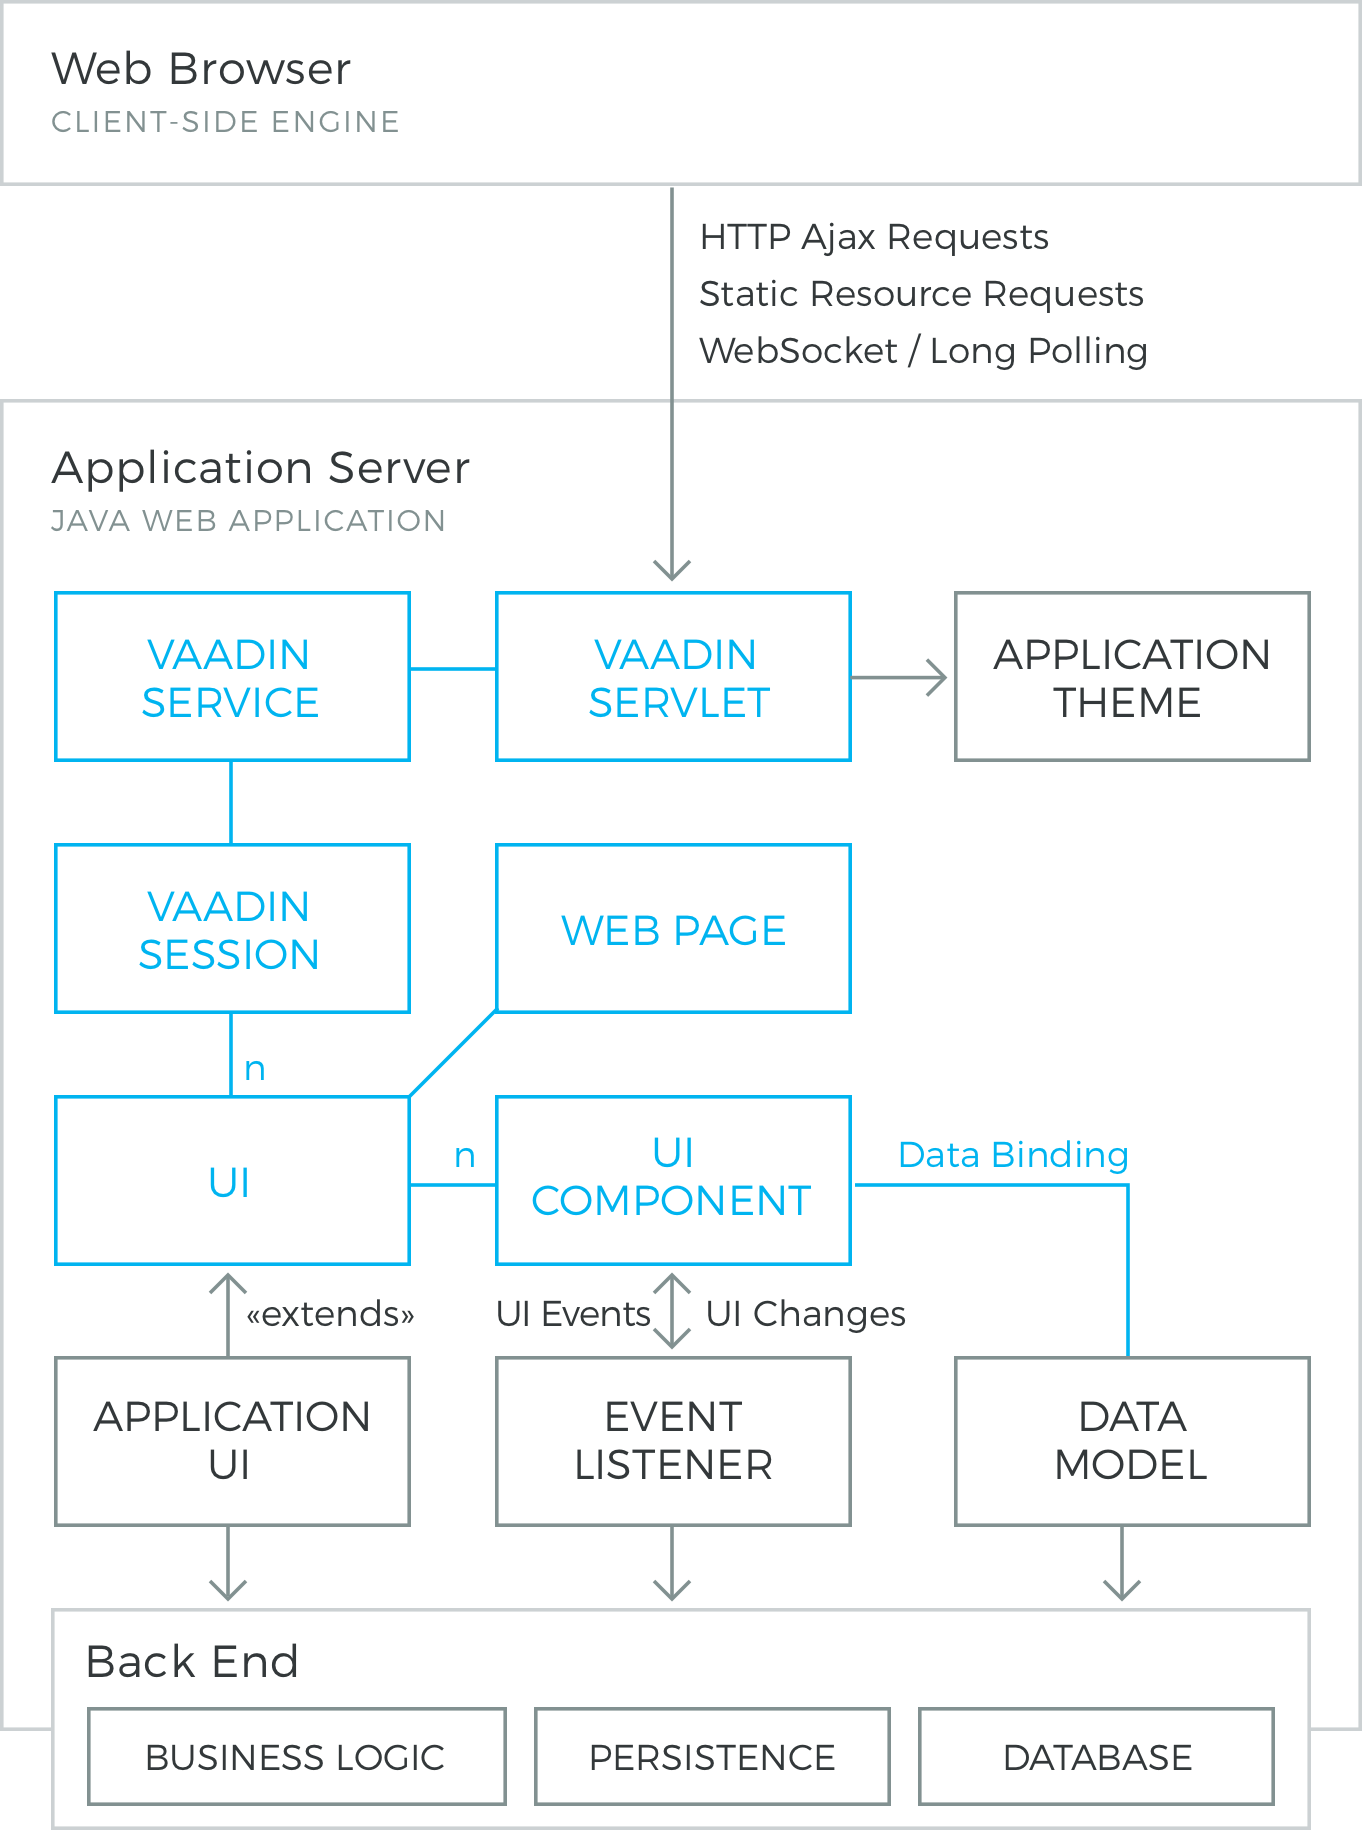
\includegraphics[width=.8\linewidth]{Images/Appendix/vaadin3.png}
			\label{fig:V3}
			\end{center}
			\end{figure}
			\paragraph{Version:} 8.1.7
			\paragraph{Advantages:}
			\begin{itemize}
				\item{}Vaadin masked many basic but complex and long aspects of Java Web programming, allowing developers to concentrate on the functionalities of Travlendar.
				\item{}Some non-functional requirements were given for granted by the framework. 
				\item{}Vaadin community is big, with a very crowded forum; it was helpful.
				\item{}Many Vaadin built-in components were available.
			\end{itemize}
			\paragraph{Drawbacks:}
			\begin{itemize}
				\item{}It was hard to make Vaadin and custom Javascript files work together.
				\item{}It took time to get confident with the environment and the high number of packages/elements.
			\end{itemize}
			\paragraph{In our project:} used to build the bones of the Application Server, both presentation and business logic.
	\subsection{Spring Boot Framework}
			\begin{figure}[H]
			\begin{center}
			
\includegraphics[width=.2\linewidth]{Images/Appendix/spring1.png}
			\label{fig:S1}
			\end{center}
			\end{figure}
		\paragraph{}Spring is framework open source for Java Web Applications. Spring Boot is the starting point for building all Spring-based applications. Spring Boot is designed to get you up and running as quickly as possible, with minimal upfront configuration of Spring: 
		\begin{itemize}
			\item{}Build anything - REST API, WebSocket, Web, Streaming, Tasks, and more.
			\item{}Simplified Security.
			\item{}Rich support for SQL and NoSQL.
			\item{}Embedded runtime support - Tomcat, Jetty, and Undertow.
			\item{}Developer productivity tools such as live reload and auto restart.
			\item{}Production-ready features such as tracing, metrics and health status.
		\end{itemize}
		\paragraph{Version:}1.5.9
		\paragraph{Advantages:}
		\begin{itemize}
			\item{}Suits well with Vaadin.
			\item{}Added more pre-build features.
		\end{itemize}
		\paragraph{Drawbacks:}
		\begin{itemize}
			\item{}It is quite complicated.
			\item{}It needed time to be understood.
		\end{itemize}
		\paragraph{In our project:}used some features, especially the ones concerning CDI, beans and database.
	\subsection{Stripe Checkout}
			\begin{figure}[H]
			\begin{center}
			
\includegraphics[width=.2\linewidth]{Images/Appendix/stripe.png}
			\label{fig:Stripe}
			\end{center}
			\end{figure}		
		\paragraph{}Stripe builds the most powerful and flexible tools for internet commerce. Whether you’re creating a subscription service, an on-demand marketplace, an e-commerce store, or a crowdfunding platform, Stripe’s meticulously-designed APIs and unmatched functionality help you create the best possible product for your users. Checkout is an embeddable payment form for desktop, tablet, and mobile devices. It works within your site—customers can pay instantly, without being redirected away to complete the transaction.
		\paragraph{Version:} 5.25
		\paragraph{Advantages:}
		\begin{itemize}
			\item{}The API has its java version: it was very easy to use.
		\end{itemize}
		\paragraph{Drawbacks:}
		\begin{itemize}
			\item{}Checkout presentation is made with a javascript file that was hard to insert in the project.
		\end{itemize}
		\paragraph{In our project:}the payment gateway module is made with the help of Stripe’s API and Checkout element.
	\subsection{SQL}
			\begin{figure}[H]
			\begin{center}
			
\includegraphics[width=.2\linewidth]{Images/Appendix/sql.png}
			\label{fig:SQL}
			\end{center}
			\end{figure}		
		\paragraph{}SQL is a domain-specific language used in programming and designed for managing data held in a relational database management system. Originally based upon relational algebra and tuple relational calculus, SQL consists of many types of statements,which may be informally classed as sublanguages, commonly: a data query language (DQL), a data definition language (DDL), data control language (DCL), and a data manipulation language (DML) . The scope of SQL includes data query, data manipulation (insert, update and delete), data definition (schema creation and modification), and data access control. Although SQL is often described as, and to a great extent is, a declarative language (4GL), it also includes procedural elements.
		\paragraph{Version:} 5.7.0
		\paragraph{Advantages:}
		\begin{itemize}
			\item{}Developers were familiar with the language.
		\end{itemize}
		\paragraph{Drawbacks:}
		\begin{itemize}
			\item{}Nowadays it is considered old technology.
		\end{itemize}
		\paragraph{In our project:} used in all the database part.
	\subsection{Java Enterprise Edition}
			\begin{figure}[H]
			\begin{center}
			
\includegraphics[width=.2\linewidth]{Images/Appendix/javaee.png}
			\label{fig:JEE}
			\end{center}
			\end{figure}		
		\paragraph{}Java Platform, Enterprise Edition (Java EE) is the standard in community-driven enterprise software. Java EE is developed using the Java Community Process, with contributions from industry experts, commercial and open source organizations, Java User Groups, and countless individuals. Each release integrates new features that align with industry needs, improves application portability, and increases developer productivity.
		\paragraph{IDE} Eclipse Oxygen and Netbeans 8.2
		\paragraph{Advantages:}
		\begin{itemize}
			\item{}Various and user-friendly IDEs.
		\end{itemize}
		\paragraph{Drawbacks:}
		\begin{itemize}
			\item{}None
		\end{itemize}
		\paragraph{In our project:} it was the development environment and basic toolkit.



		
			
.
		
\end{document}